\documentclass[11pt]{article}
\usepackage[margin=1in]{geometry}
\usepackage{amsmath}
\usepackage{amssymb}
\usepackage{booktabs}
\usepackage{graphicx}
\usepackage{float}
\usepackage{caption}
\usepackage[hidelinks]{hyperref}

\newcommand{\invlogit}{\operatorname{logit}^{-1}}
\newcommand{\code}[1]{\texttt{#1}}

\graphicspath{{Plots_C/Fit_Plots_C/}}

\title{Model C Fit to the Real Data}
\author{Vera Schroeder}
\date{October 2026}

\begin{document}

\maketitle

\section{Summary}

Model C (hierarchical over sessions, one group per hand, distractor amplitude as a
covariate) was fit to all 12{,}937 trials of the Sirius data (42 sessions). The main
results:

\begin{itemize}
  \item \textbf{The PSE shift grows with distractor amplitude.} The hand-level
        distractor coefficient is clearly positive, $\mu_{\beta_2} = 0.90$
        [0.71, 1.09] (left) and 1.18 [0.99, 1.37] (right). For a typical session
        the bimanual PSE lies 1.2 (left) and 1.7 (right) $\mu m$ below the unimanual
        one with a 6 $\mu m$ distractor, and 6.6 and 8.9 $\mu m$ below with 32
        $\mu m$. Averaged over the 42 sessions the shift is $-4.5$ $\mu m$ (left) and
        $-5.7$ $\mu m$ (right), close to Model B's estimates.
  \item \textbf{The fit is reliable but the model misfits in specific places.} The
        sampler converged without problems. However, the bimanual trials at the
        weakest stimuli contain more ``high'' responses than Model C predicts, and
        LOO prefers Model B by 37.1 (SE 11.9), with most of the difference at the
        6 and 12 $\mu m$ stimuli.
  \item \textbf{The misfit follows from three assumptions of Model C}: unimanual and
        bimanual trials share their lapse rates, they share their slope, and the
        PSE shift is proportional to the distractor amplitude, so it shrinks to 0
        for a weak distractor. For the right hand, the 6 $\mu m$ sessions shift by
        3.9 $\mu m$ on average under Model B but only 1.7 $\mu m$ under Model C.
  \item The amplitude dependence itself is robust, but its size at small amplitudes,
        and the shared lapse rates and slopes, should be revisited before Model C's
        estimates are used for inference (Section~\ref{sec:conclusions}).
\end{itemize}

Every figure and number in this report is produced by \code{Main\_Analysis\_C.py};
the cell ``Numbers for Fit\_C\_Report.tex'' prints the numbers that the earlier
cells do not. All intervals are 95\% highest density intervals (HDIs). PSE and JND
are in micrometres of stimulus amplitude: $\text{PSE}_{\mu m} = 28 + 14.63\,\text{PSE}$
and $\text{JND}_{\mu m} = 14.63\,\text{JND}$, where 28 and 14.63 are the mean and sd of
the 8 amplitude levels.

\section{Model and Fit}

The model is the one described in the Model C convergence report. For hand $j$ and
session $s$,
\[
  \psi(x, d) = \gamma_{h,js} + (1 - \gamma_{h,js} - \gamma_{l,js})\,
  \invlogit\big(\beta_{0,js} + \beta_{1,js}\, x + \beta_{2,js}\, d\big),
\]
where $x$ is the standardized stimulus amplitude and $d$ the distractor amplitude
divided by 14.63 ($d = 0$ on unimanual trials; every session uses a single distractor
amplitude on its bimanual trials). The five session parameters are drawn from
hand-level normal (for $\beta$) and logit-normal (for $\gamma$) distributions. The
priors on $\beta_0$, $\beta_1$ and the lapse rates are those of Model B, and
$\mu_{\beta_2} \sim \mathcal{N}(0, 1)$, $\sigma_{\beta_2} \sim \text{HalfNormal}(1)$.

Because $\beta_2 d$ only shifts the curve, the PSE shift of a session is
$-\beta_2 d_s / \beta_1$ standardized units, and its JND and lapse rates are the same
in both conditions.

The fit used NUTS with 4 chains of 1000 tuning and 5000 kept draws (20{,}000 draws in
total) and took 9 minutes. The data have 3{,}230--3{,}237 trials in each hand
$\times$ condition cell.

\subsection{Sampling diagnostics}

There were 2 divergences in the 20{,}000 draws, and the tree depth never exceeded 5.
All 1{,}300 variables, including the raw sampler variables, have $\hat{R} = 1.000$,
bulk ESS $\ge 3{,}410$ and tail ESS $\ge 5{,}231$. Unlike Model B, whose raw
\code{z\_sig\_b0} variables showed $\hat{R}$ warnings from an unidentified sign,
Model C defines its HalfNormal sds directly, so no such warning appears.

Figures~\ref{fig:trace_sess}--\ref{fig:trace_gamh} show trace plots for a few
parameters: the left hand's session parameters in session 04-13 (12 $\mu m$
distractor; the session whose curves are shown below) and 05-12 (32 $\mu m$), the
hyperparameters of $\beta_2$, and the lapse rate $\gamma_h$ with its hyperparameters.
The four chains overlap and mix quickly, including for $\sigma_{\gamma_h}$, which
piles up against 0. The gray ticks on the axes mark the 2 divergent draws; they lie
in no particular region of the posterior.

\begin{figure}[H]
\centering
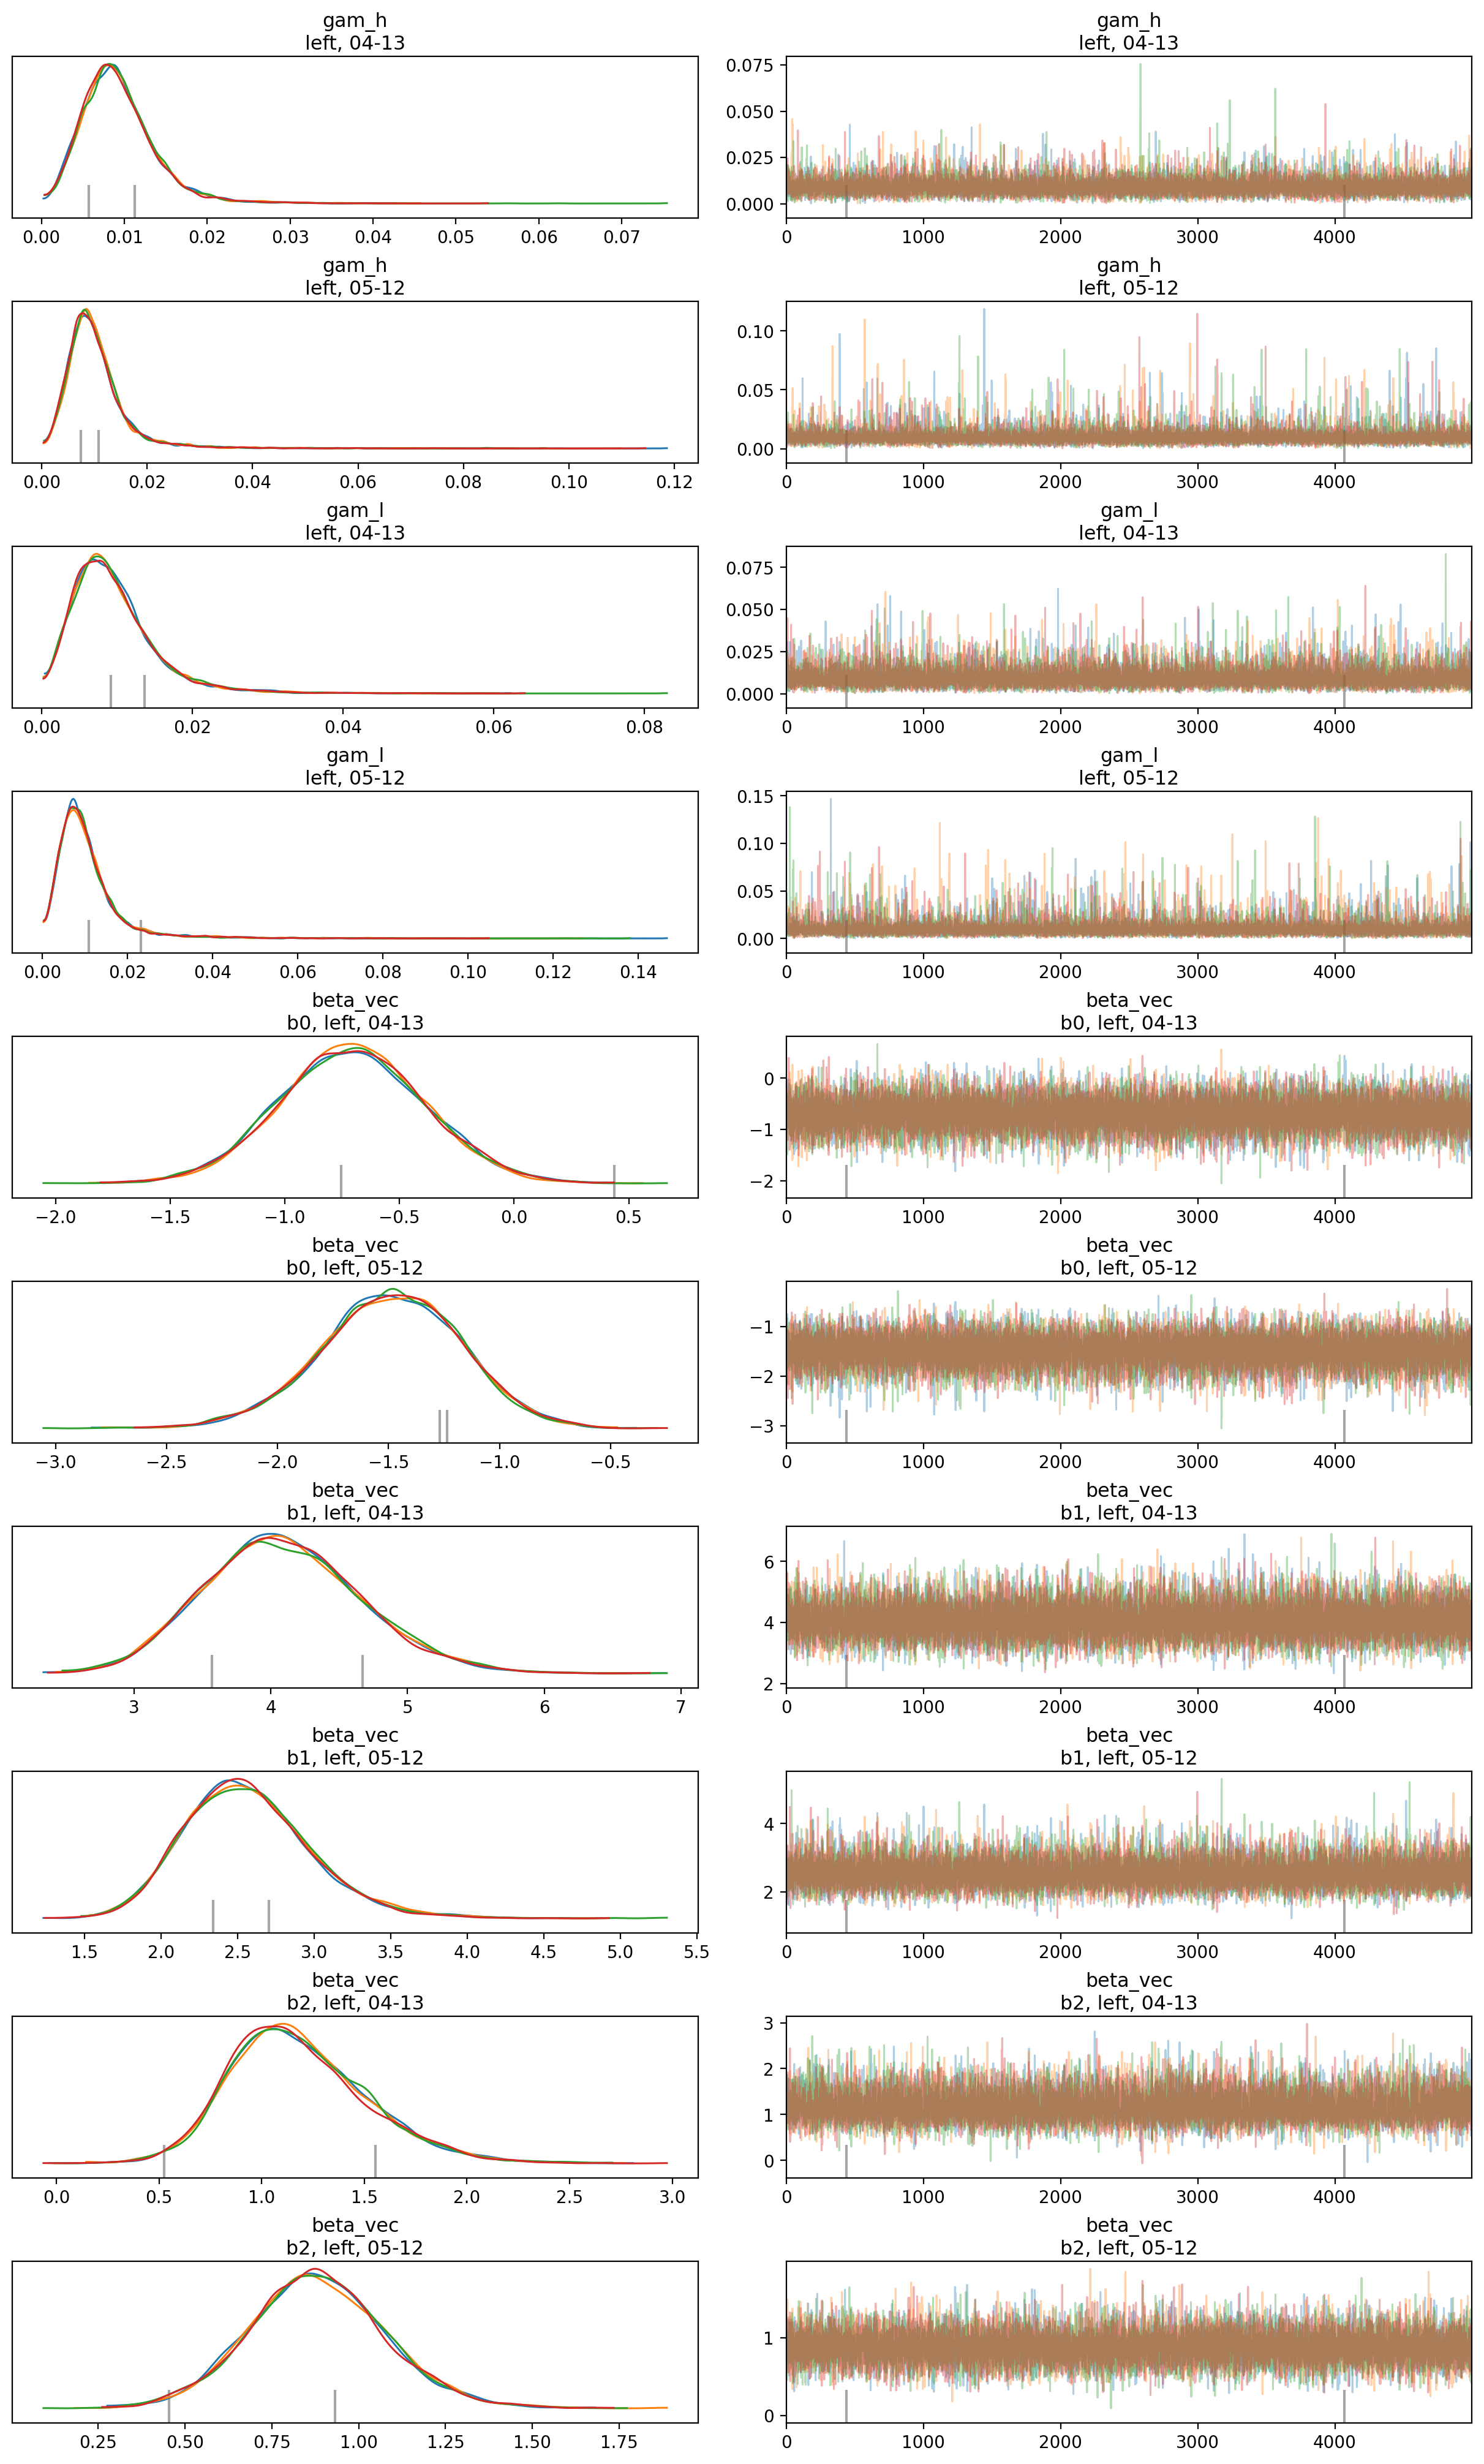
\includegraphics[height=0.8\textheight]{trace_session_params_left.png}
\caption{Trace plots (left: density per chain; right: draws per chain) of the left
hand's session-level $\gamma_h$, $\gamma_l$, $\beta_0$, $\beta_1$ and $\beta_2$ in
sessions 04-13 and 05-12.}
\label{fig:trace_sess}
\end{figure}

\begin{figure}[H]
\centering
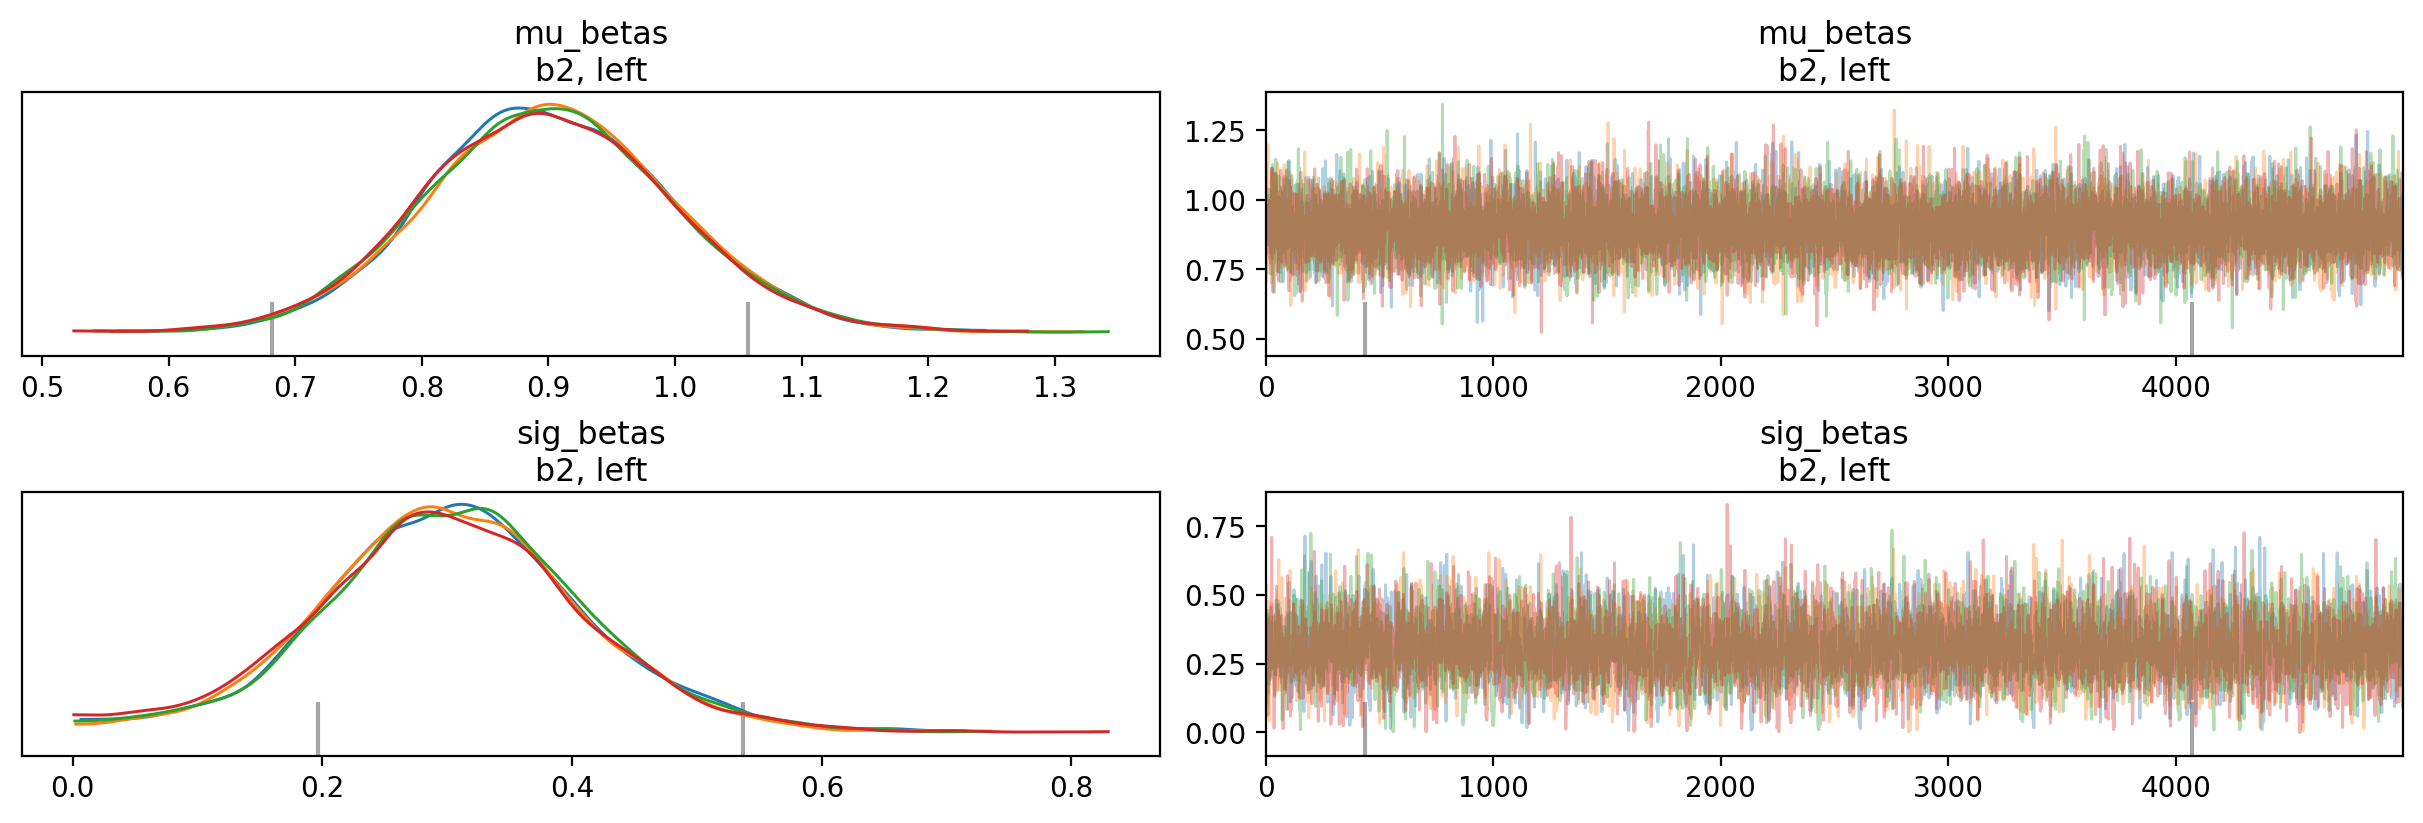
\includegraphics[width=0.9\textwidth]{trace_b2_hyper_left.png}
\caption{Trace plots of the left hand's $\mu_{\beta_2}$ and $\sigma_{\beta_2}$.}
\label{fig:trace_b2}
\end{figure}

\begin{figure}[H]
\centering
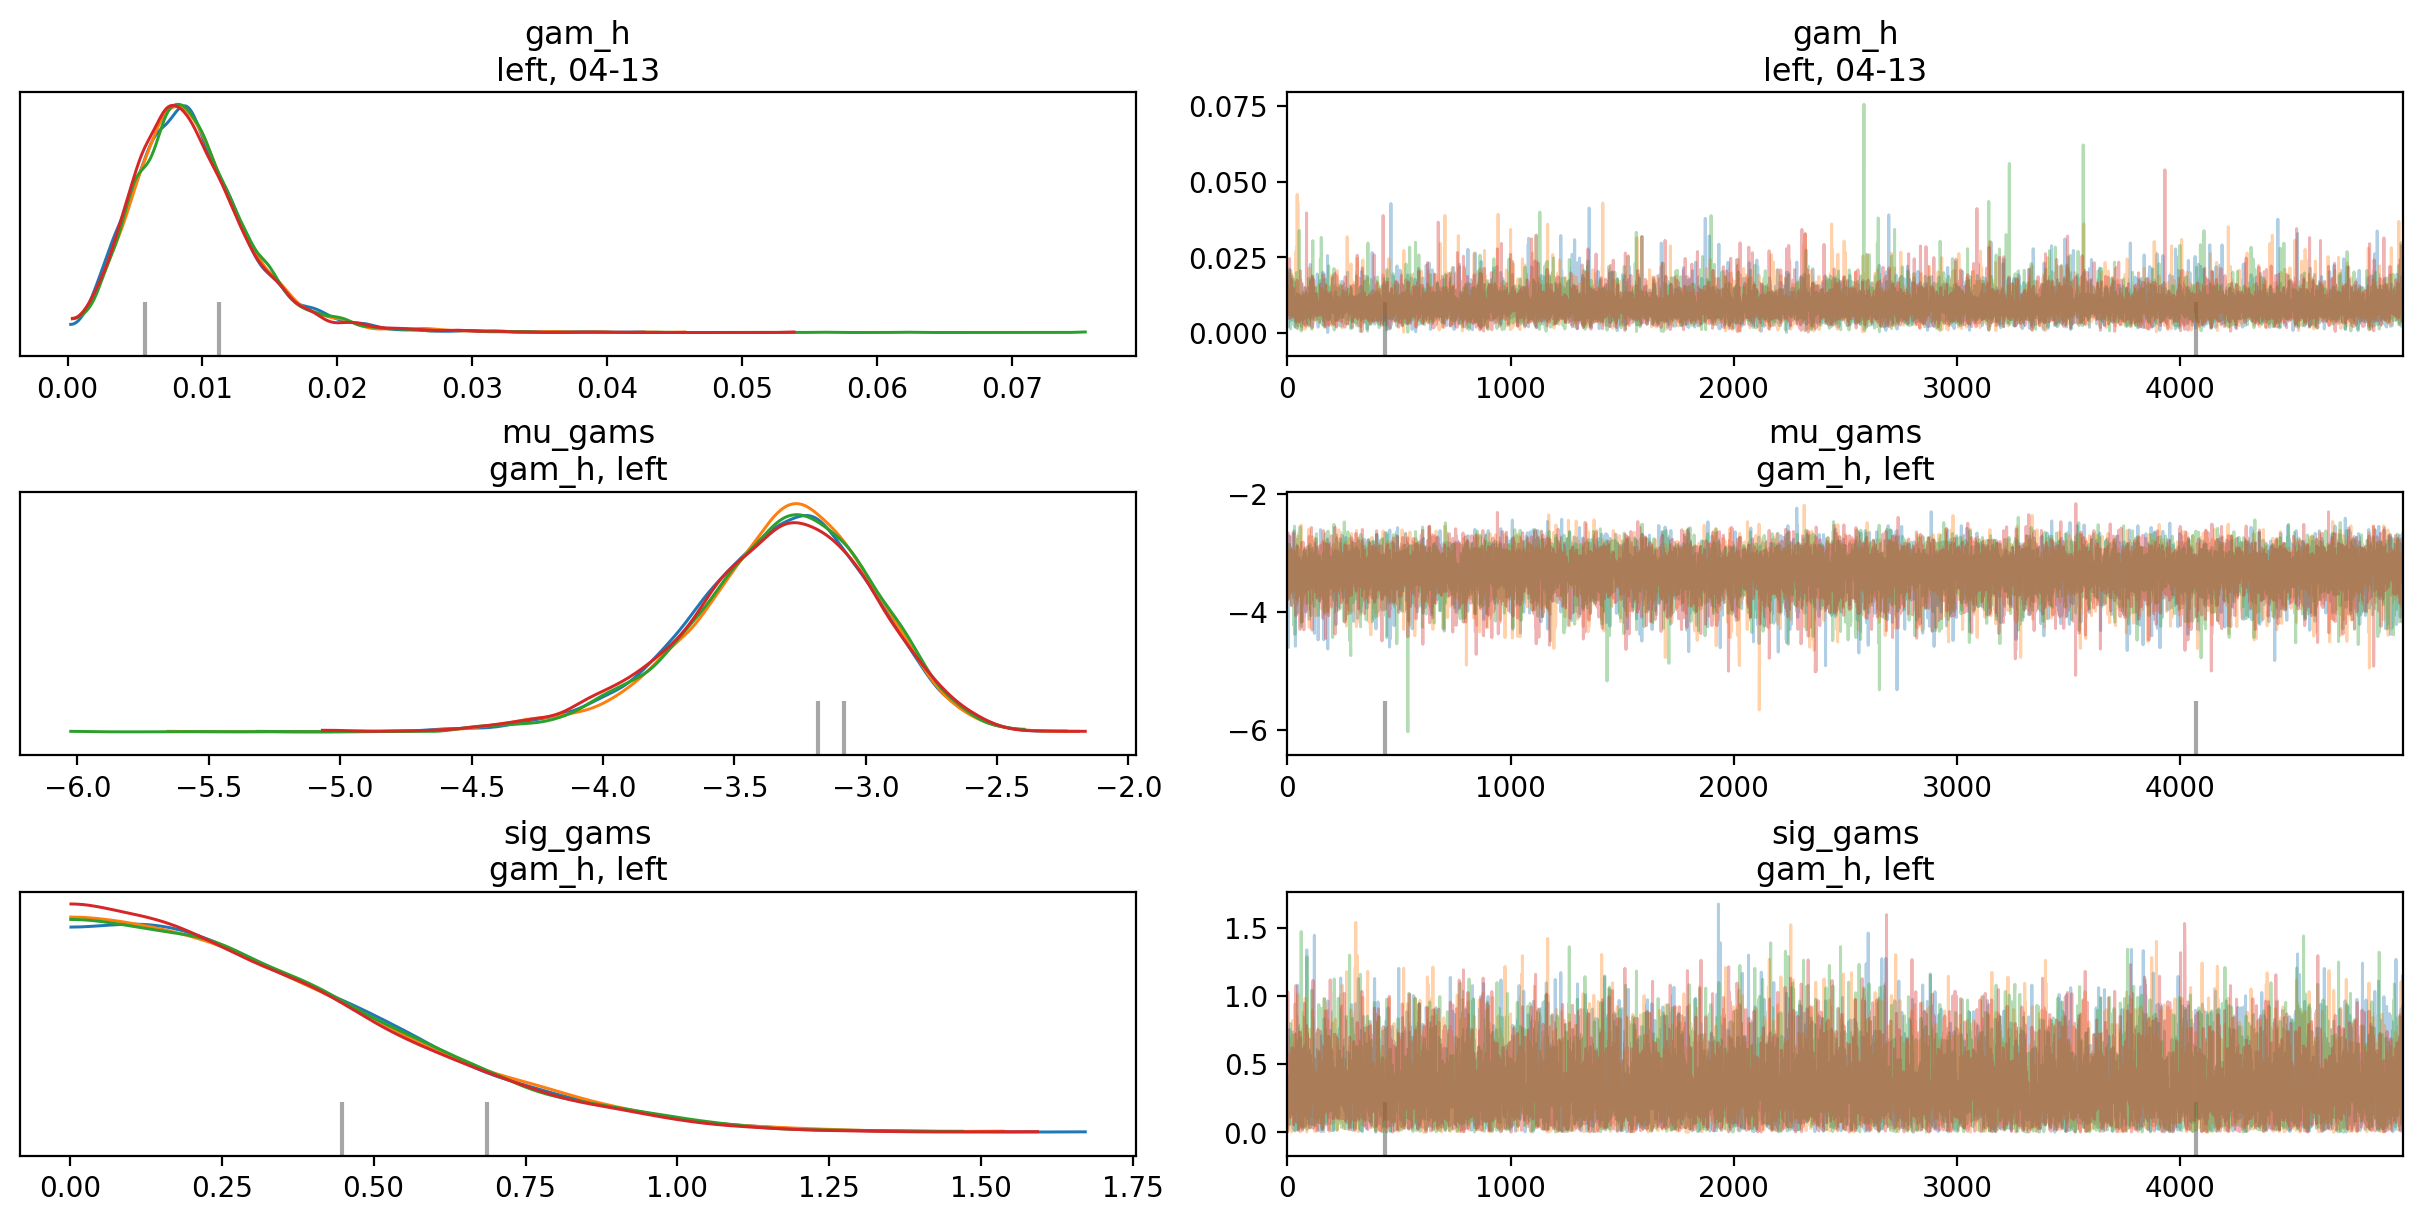
\includegraphics[width=0.9\textwidth]{trace_gam_h_hyper_left.png}
\caption{Trace plots of the left hand's $\gamma_h$ on 04-13 and of the hyperparameters
$\mu_{\gamma_h}$ and $\sigma_{\gamma_h}$ it is drawn from.}
\label{fig:trace_gamh}
\end{figure}

\subsection{Posterior predictive check}
\label{sec:ppc}

\begin{figure}[H]
\centering
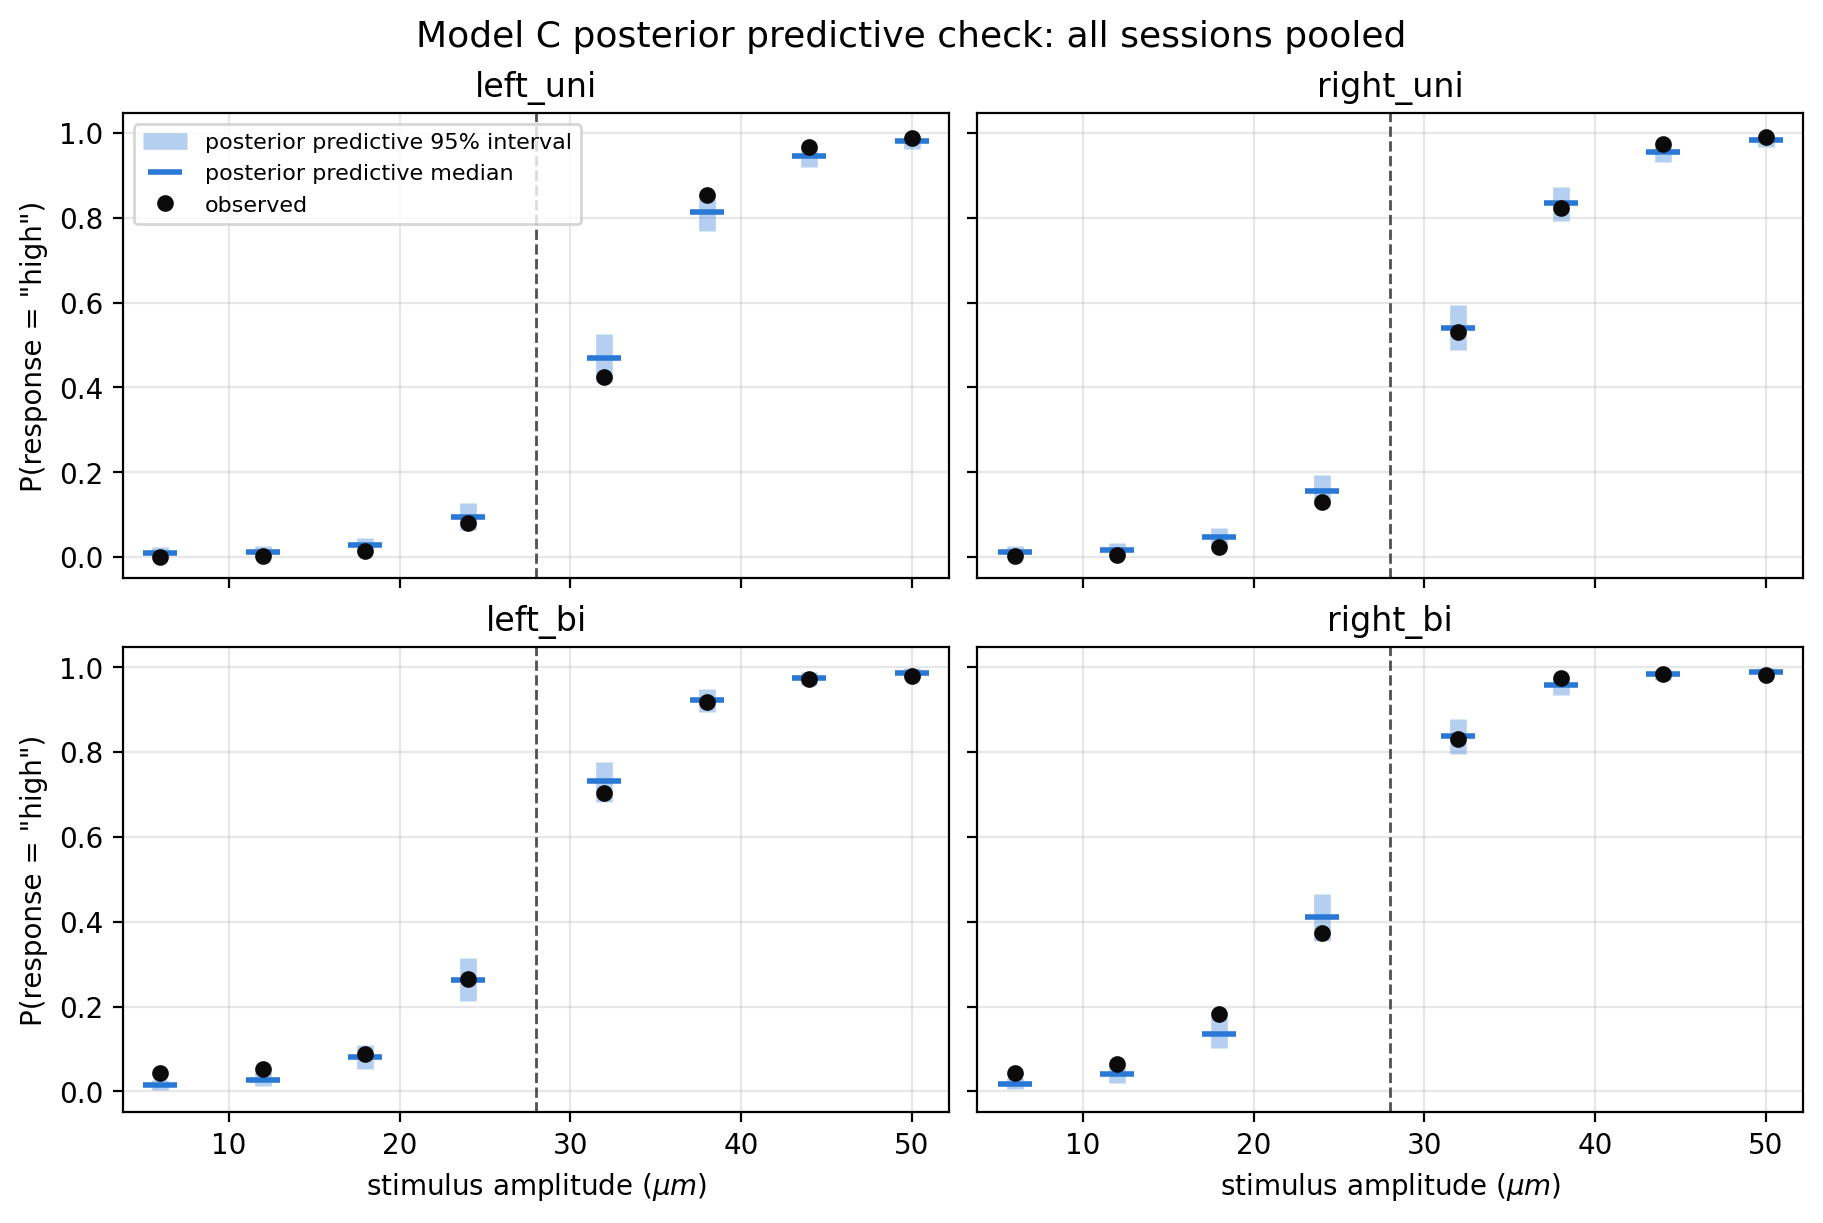
\includegraphics[width=0.85\textwidth]{ppc_pooled_by_stimulus.png}
\caption{Observed proportion of ``high'' responses at each amplitude, pooled over
sessions (black), against the posterior predictive median and 95\% interval (blue),
by hand and condition. The dashed line is the trained threshold of 28 $\mu m$.}
\label{fig:ppc}
\end{figure}

Of the 32 hand $\times$ condition $\times$ amplitude proportions, 26 lie inside their
95\% posterior predictive intervals (Figure~\ref{fig:ppc}). The six outside are all at
the weak end of the stimulus range (Table~\ref{tab:ppc}): on bimanual trials Model C
predicts too few ``high'' responses at 6--18 $\mu m$, and on left unimanual trials at
6 $\mu m$ it predicts a few where the monkey gave none.

\begin{table}[H]
\centering
\caption{Proportions outside their 95\% posterior predictive interval.}
\label{tab:ppc}
\begin{tabular}{llcccc}
\toprule
hand & condition & amplitude ($\mu m$) & observed & predicted median & 95\% interval \\
\midrule
left  & unimanual & 6  & 0.000 & 0.010 & [0.002, 0.025] \\
left  & bimanual  & 6  & 0.042 & 0.015 & [0.002, 0.027] \\
left  & bimanual  & 12 & 0.052 & 0.028 & [0.012, 0.045] \\
right & bimanual  & 6  & 0.042 & 0.017 & [0.005, 0.032] \\
right & bimanual  & 12 & 0.065 & 0.040 & [0.020, 0.062] \\
right & bimanual  & 18 & 0.183 & 0.136 & [0.101, 0.175] \\
\bottomrule
\end{tabular}
\end{table}

This is the pattern expected if the distractor raises the lapse rate $\gamma_h$ but
the model can only use one lapse rate for both conditions. The fitted typical lapse
rates ($\gamma_h = 0.009$ and 0.011, Table~\ref{tab:pop}) lie between the near-zero
unimanual and the higher bimanual rates that Model B estimates separately: too high
for unimanual trials and too low for bimanual ones.

\paragraph{Within single sessions.}
Each session $\times$ hand $\times$ condition $\times$ amplitude cell holds about 10
trials. Of the 1{,}344 cells, 1{,}331 (99.0\%) have their observed count of ``high''
inside the 95\% posterior predictive interval, and 2.0\% and 1.7\% of the PIT values
are below 0.025 and above 0.975, against 2.5\% each for a calibrated model
(Figure~\ref{fig:ppc_sessions}). Each cell's interval comes from a model fit partly to
that same cell, so this is a check for gross misfit, and none appears: the lowest
coverage, 0.93, is for right-hand bimanual trials at 6 $\mu m$. The misfit of
Table~\ref{tab:ppc} is systematic but small in any one session, and only shows when the
sessions are pooled.

\begin{figure}[H]
\centering
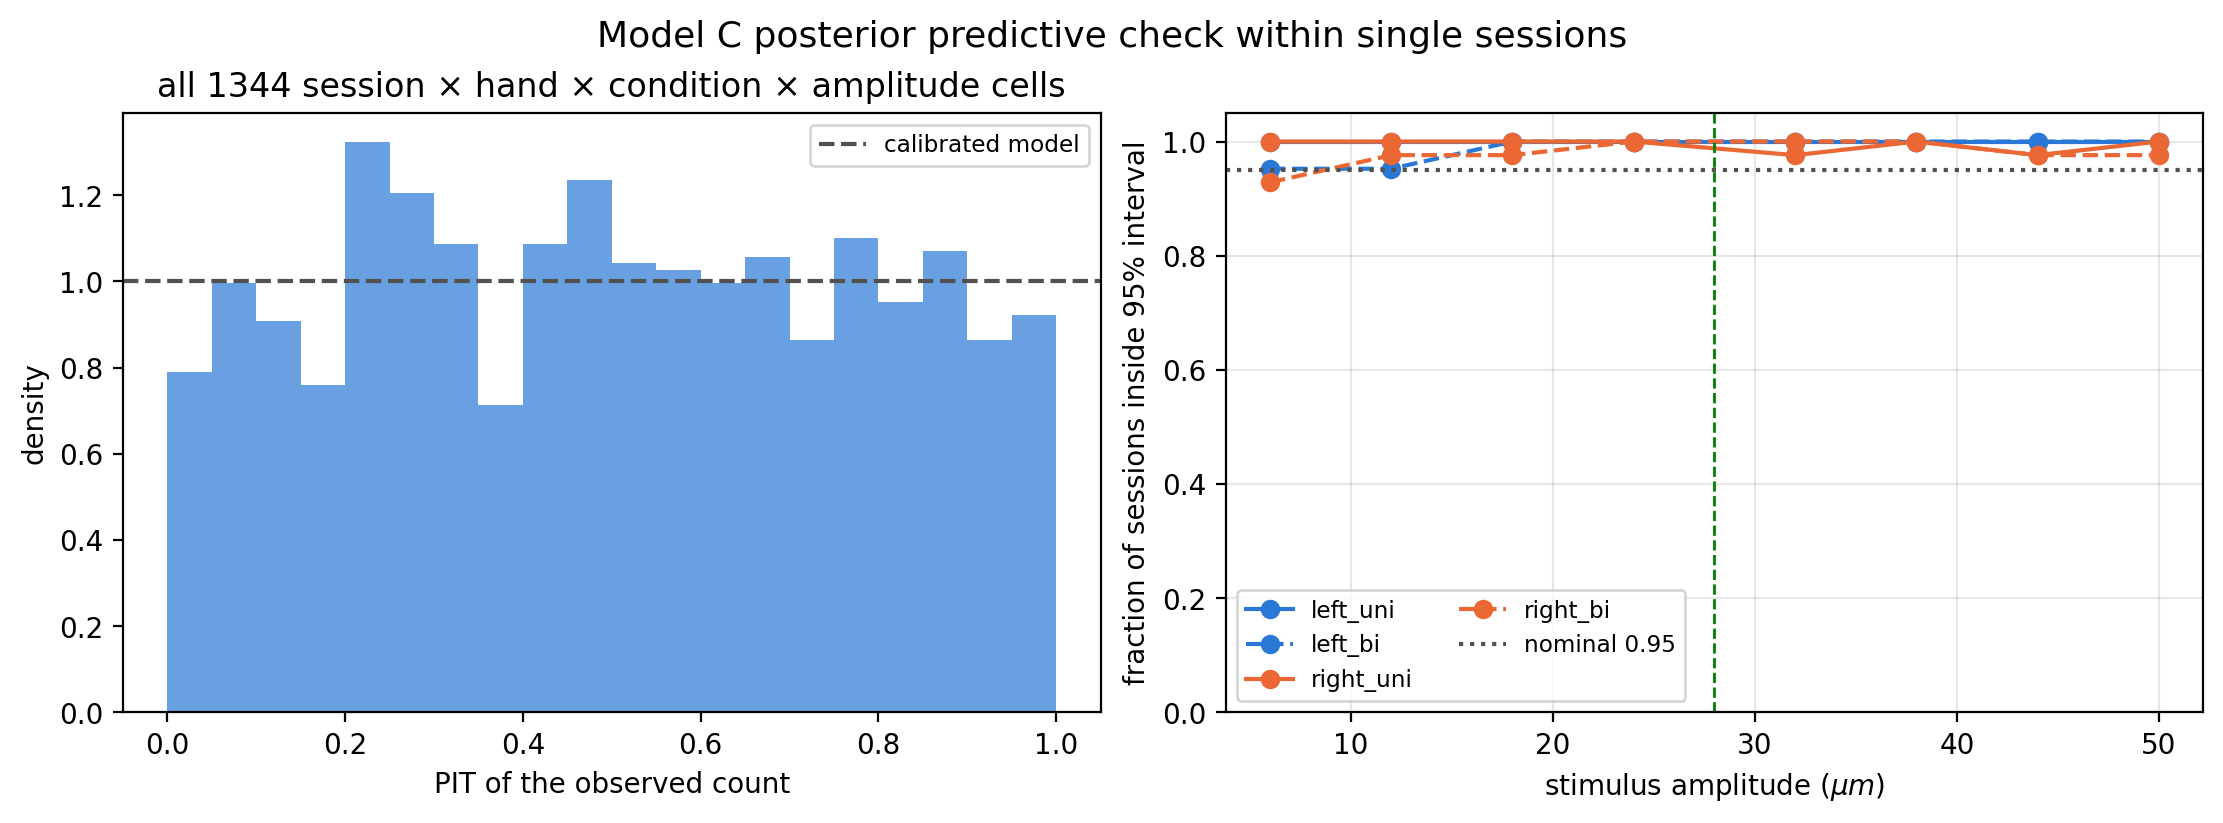
\includegraphics[width=\textwidth]{ppc_session_cells.png}
\caption{Posterior predictive check within single sessions. Left: PIT values of the
observed number of ``high'' responses in each session $\times$ hand $\times$ condition
$\times$ amplitude cell (flat at 1 for a calibrated model). Right: fraction of the 42
sessions whose observed count lies inside its 95\% predictive interval.}
\label{fig:ppc_sessions}
\end{figure}

\begin{figure}[H]
\centering
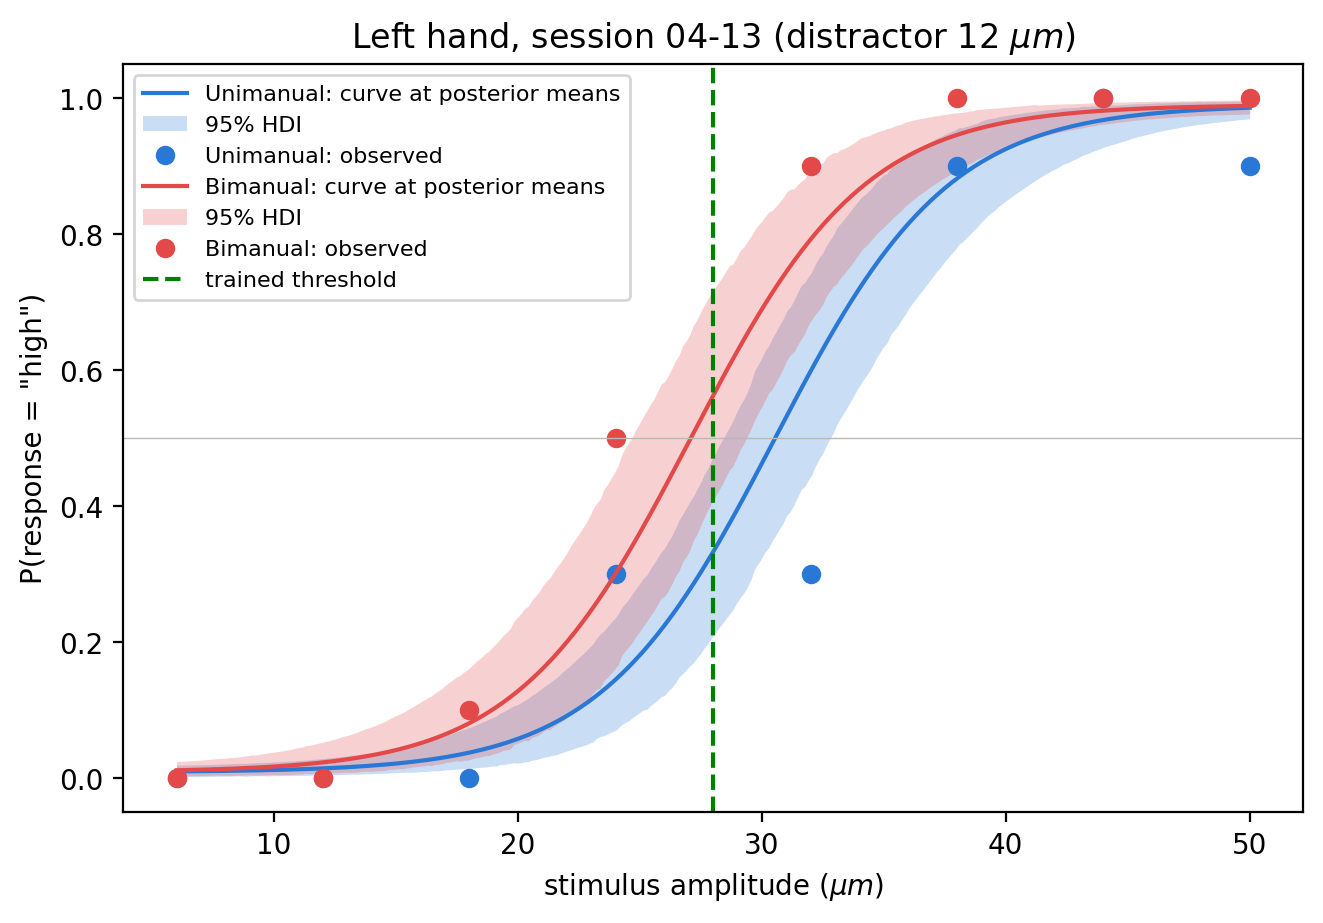
\includegraphics[width=0.48\textwidth]{curves_left_04-13.png}\hfill
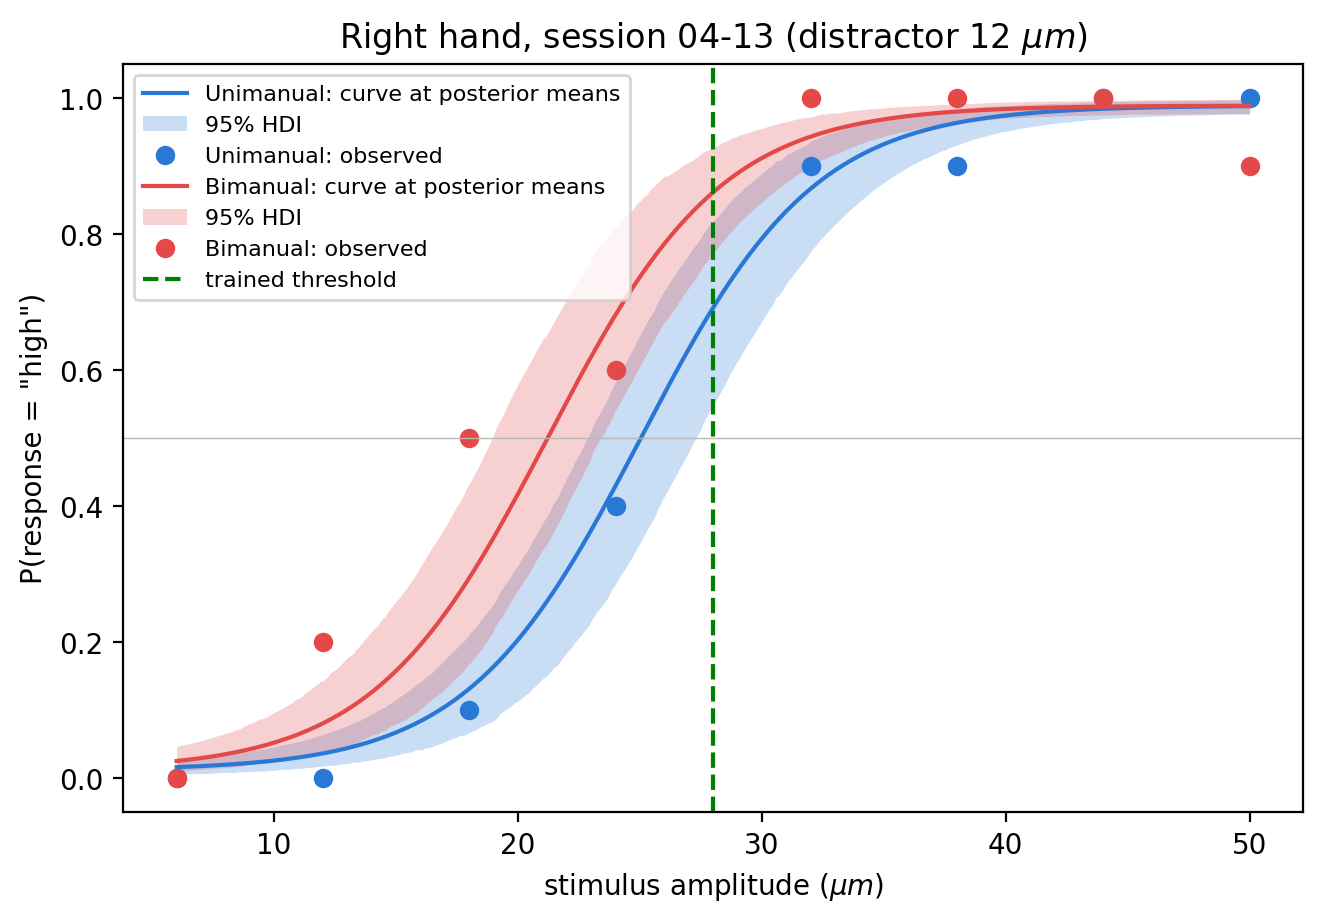
\includegraphics[width=0.48\textwidth]{curves_right_04-13.png}
\caption{Fitted psychometric curves for session 04-13 (12 $\mu m$ distractor): the
curve at the posterior means of the parameters, the pointwise 95\% HDI of the curve,
and the observed proportions of ``high'' responses (9--10 trials per point).
Unimanual in blue, bimanual in red; the dashed line is the trained threshold.}
\label{fig:curves}
\end{figure}

Figure~\ref{fig:curves} shows the fit in one session, 04-13, the session shown in
the Model B report. The two curves of a hand have the same slope and asymptotes and
differ only in position. The bimanual curve lies to the left of the unimanual one,
with session PSEs of 30.6 (unimanual) and 27.1 (bimanual) $\mu m$ for the left hand
and 25.0 and 21.2 $\mu m$ for the right. With about 10 trials per point the observed
proportions scatter around the curves; single stray points, such as the left
unimanual proportion of 0.3 at 32 $\mu m$, pull the curve only partly towards them.

\begin{figure}[H]
\centering
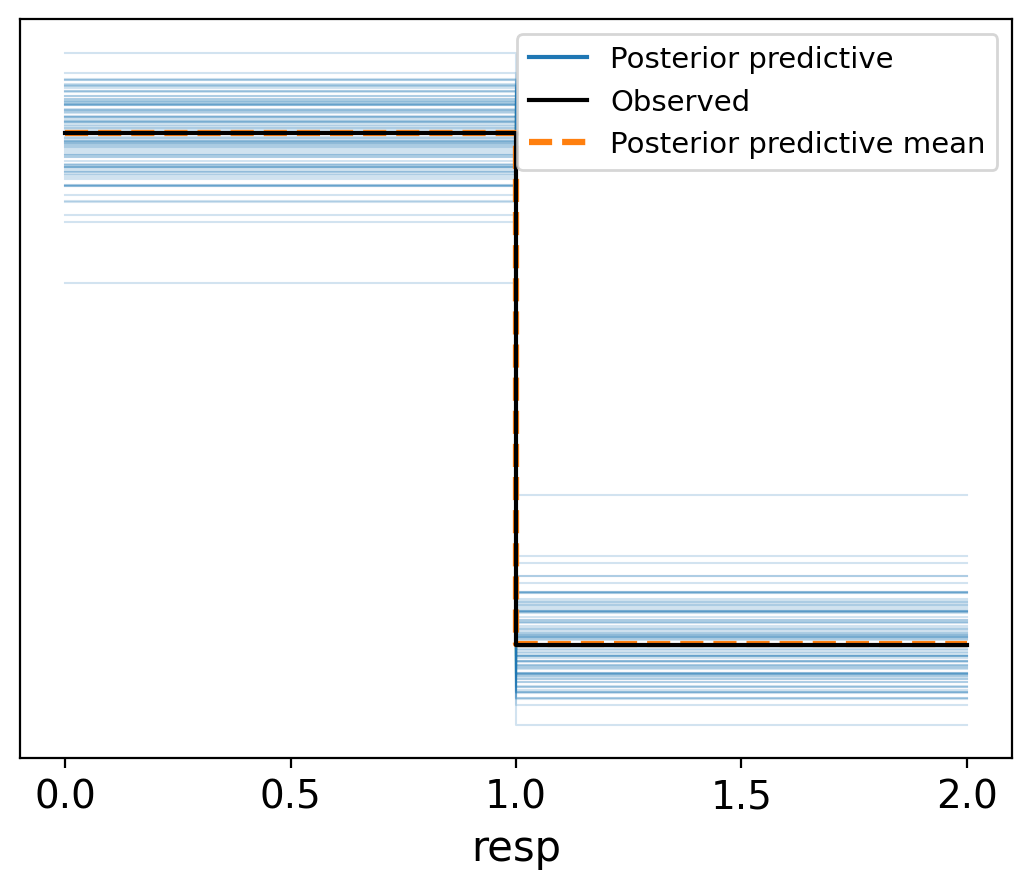
\includegraphics[width=0.55\textwidth]{ppc_arviz_resp.png}
\caption{ArviZ posterior predictive check of the responses (0 = ``low'',
1 = ``high''), pooled over all trials: observed (black), 100 posterior predictive
draws (blue) and their mean (orange dashed).}
\label{fig:ppc_arviz}
\end{figure}

The overall proportion of ``high'' responses is reproduced
(Figure~\ref{fig:ppc_arviz}); for binary data this check is coarse, and
Figure~\ref{fig:ppc} is the more informative one.

\section{Population-level Results}

\begin{table}[H]
\centering
\caption{Hand-level hyperparameters: posterior mean [95\% HDI]. The lapse-rate
hyperparameters are on the logit scale.}
\label{tab:hyper}
\begin{tabular}{lcc}
\toprule
 & left & right \\
\midrule
$\mu_{\beta_0}$ & $-1.30$ [$-1.56$, $-1.04$] & $-0.92$ [$-1.29$, $-0.55$] \\
$\mu_{\beta_1}$ & 4.39 [3.95, 4.85] & 4.25 [3.92, 4.62] \\
$\mu_{\beta_2}$ & 0.90 [0.71, 1.09] & 1.18 [0.99, 1.37] \\
$\sigma_{\beta_0}$ & 0.60 [0.39, 0.81] & 1.07 [0.79, 1.36] \\
$\sigma_{\beta_1}$ & 0.90 [0.57, 1.26] & 0.35 [0.00, 0.69] \\
$\sigma_{\beta_2}$ & 0.30 [0.08, 0.51] & 0.23 [0.00, 0.45] \\
$\mu_{\gamma_h}$ & $-3.33$ [$-4.07$, $-2.69$] & $-3.11$ [$-3.91$, $-2.43$] \\
$\mu_{\gamma_l}$ & $-3.42$ [$-4.36$, $-2.60$] & $-3.41$ [$-4.18$, $-2.67$] \\
$\sigma_{\gamma_h}$ & 0.34 [0.00, 0.82] & 0.34 [0.00, 0.82] \\
$\sigma_{\gamma_l}$ & 0.40 [0.00, 0.96] & 0.47 [0.00, 1.03] \\
\bottomrule
\end{tabular}
\end{table}

\begin{table}[H]
\centering
\caption{A typical session (all parameters at their hand-level means): unimanual
PSE, JND and lapse rates, posterior mean [95\% HDI]. The JND and lapse rates are the
same on bimanual trials in Model C.}
\label{tab:pop}
\begin{tabular}{lcc}
\toprule
 & left & right \\
\midrule
PSE, unimanual ($\mu m$) & 32.34 [31.51, 33.17] & 31.15 [29.92, 32.40] \\
JND ($\mu m$) & 3.75 [3.39, 4.11] & 3.88 [3.59, 4.19] \\
$\gamma_h$ & 0.0091 [0.0033, 0.0147] & 0.0113 [0.0042, 0.0189] \\
$\gamma_l$ & 0.0086 [0.0023, 0.0155] & 0.0085 [0.0029, 0.0143] \\
\bottomrule
\end{tabular}
\end{table}

The unimanual PSE of a typical session lies 4.3 (left) and 3.2 (right) $\mu m$ above
the trained threshold of 28 $\mu m$ (Table~\ref{tab:pop}). The sessions differ in their bias
($\sigma_{\beta_0} = 0.60$ and 1.07) and, for the left hand, in their slope
($\sigma_{\beta_1} = 0.90$): the left-hand session JNDs range from 2.95 to
6.59 $\mu m$, the right-hand ones only from 3.65 to 4.31 $\mu m$. As in Model B and in
Model C's convergence study, $\sigma_{\gamma_h}$ and $\sigma_{\gamma_l}$ are not identified;
their posteriors largely reflect the prior.

The data determine all five typical-session quantities rather than the priors:
the posterior sd is 4.5--6.6\% of the prior sd for the unimanual PSE, 5.9--7.3\% for
the JND, 9--12\% for the lapse rates and 9.6--9.7\% for $\mu_{\beta_2}$
(Figures~\ref{fig:pop_pse}--\ref{fig:pop_b2}).

\begin{figure}[H]
\centering
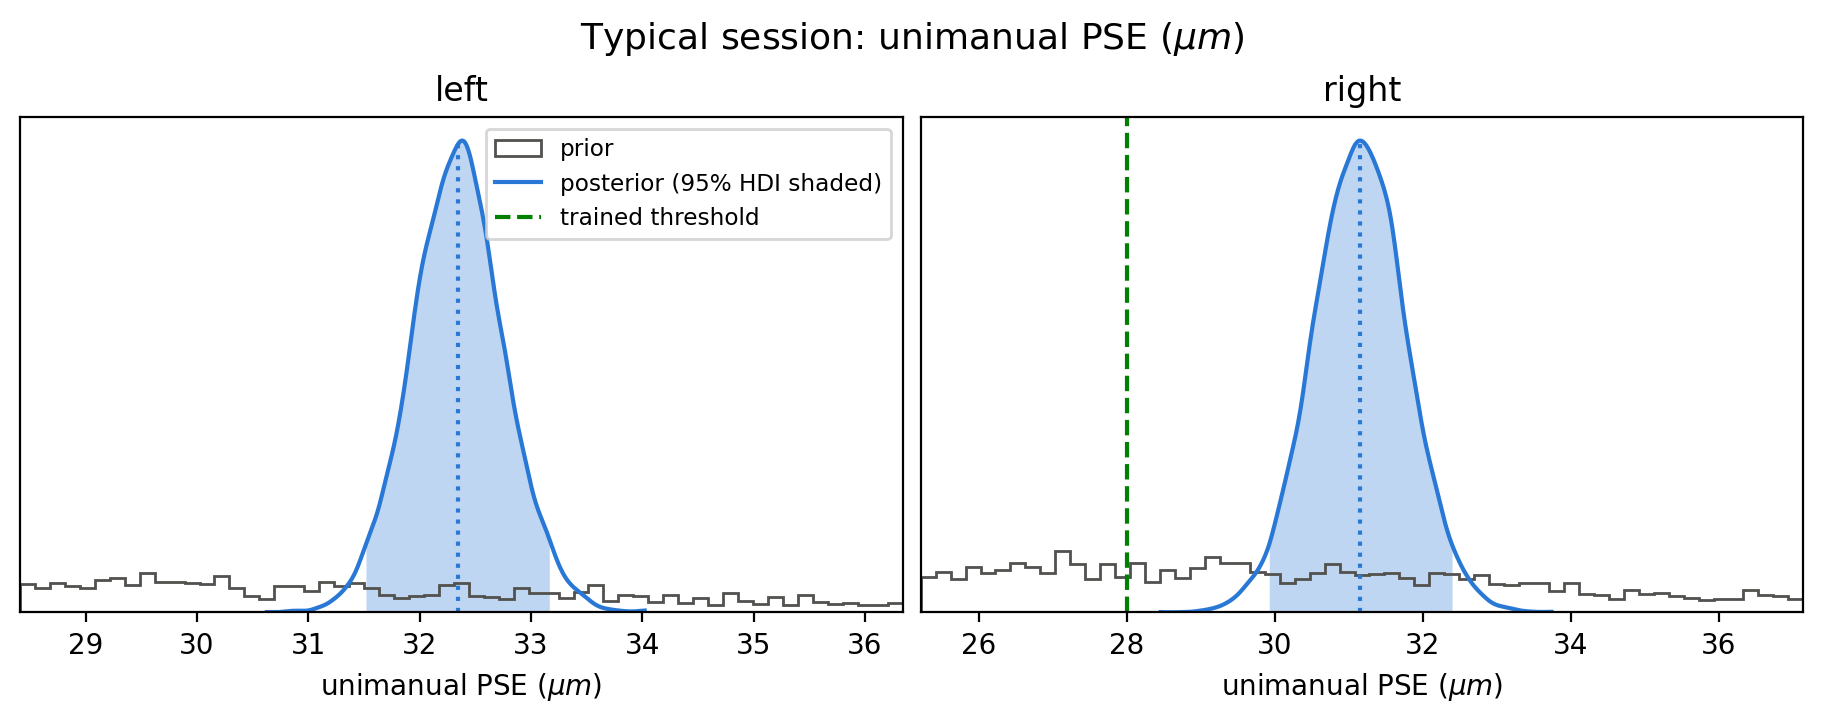
\includegraphics[width=0.8\textwidth]{population_PSE_prior_posterior.png}
\caption{Prior (gray) and posterior (blue) of a typical session's unimanual PSE.}
\label{fig:pop_pse}
\end{figure}

\begin{figure}[H]
\centering
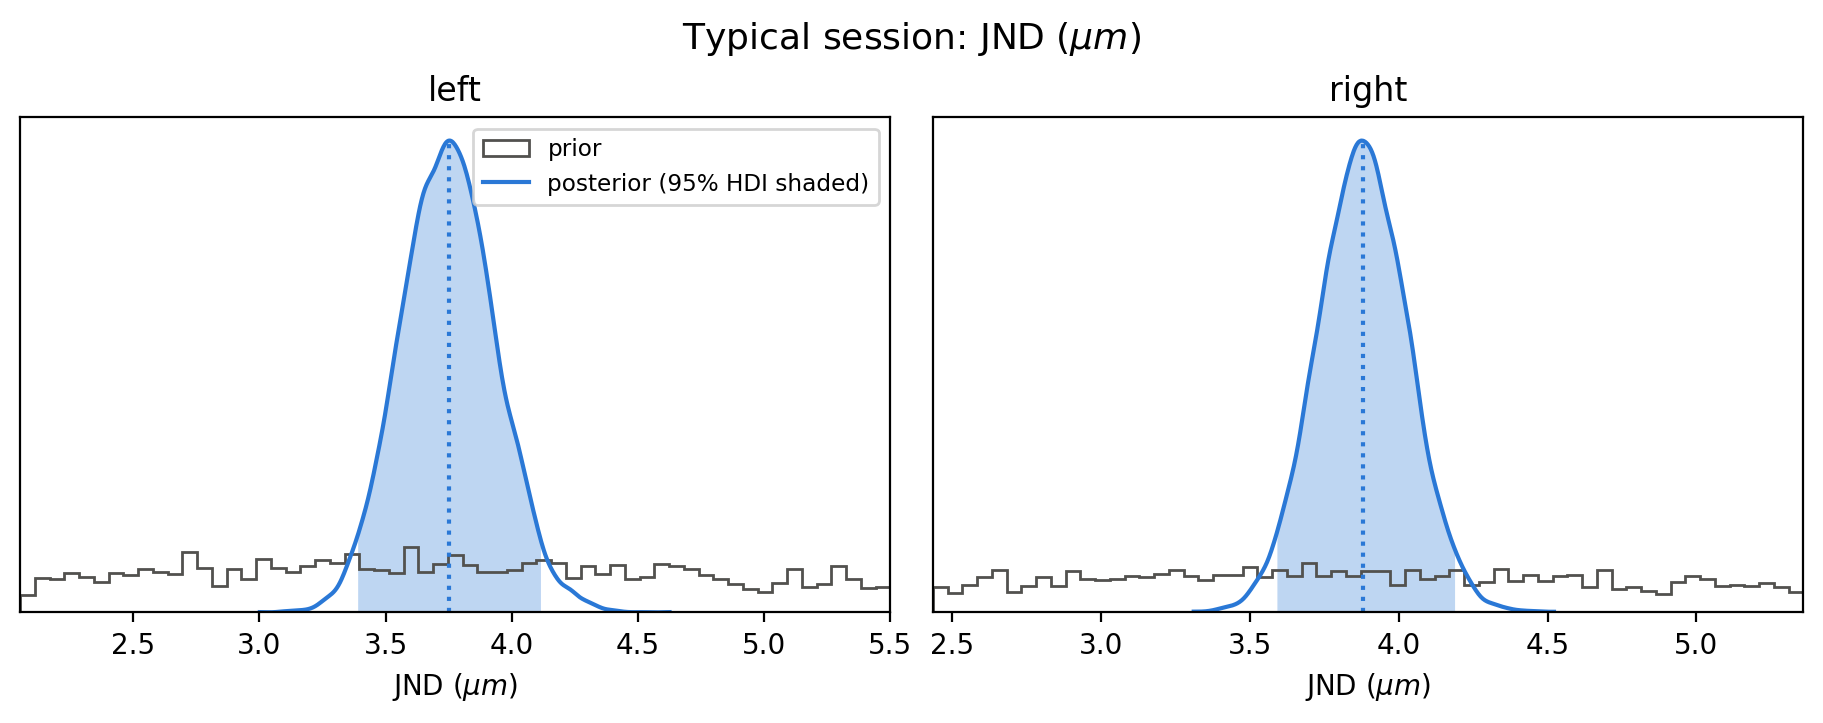
\includegraphics[width=0.8\textwidth]{population_JND_prior_posterior.png}
\caption{Prior (gray) and posterior (blue) of a typical session's JND, the same in
both conditions.}
\end{figure}

\begin{figure}[H]
\centering
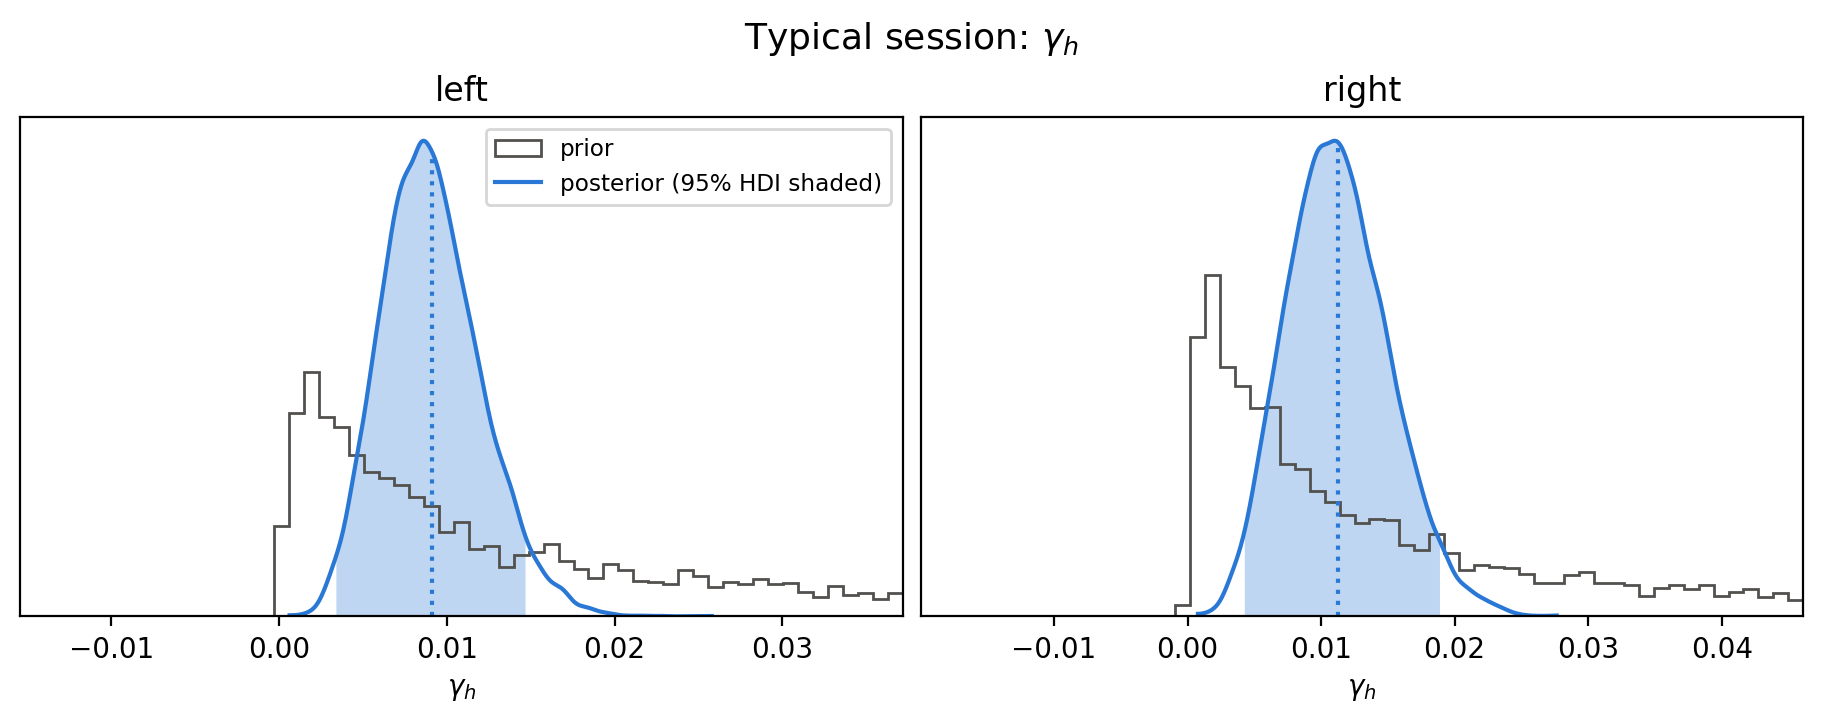
\includegraphics[width=0.8\textwidth]{population_gamh_prior_posterior.png}
\caption{Prior (gray) and posterior (blue) of a typical session's $\gamma_h$.}
\end{figure}

\begin{figure}[H]
\centering
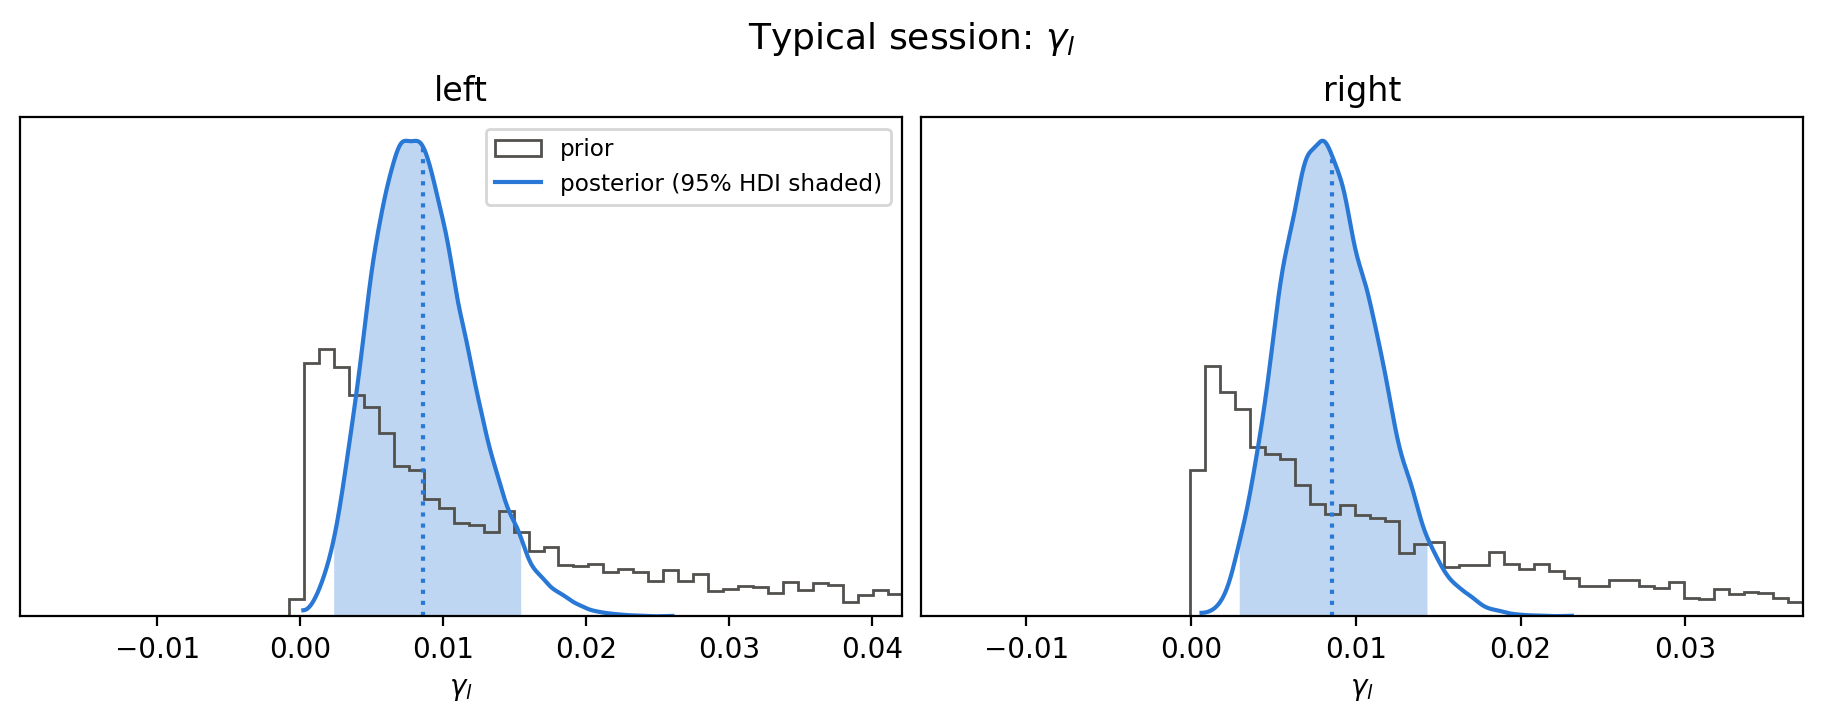
\includegraphics[width=0.8\textwidth]{population_gaml_prior_posterior.png}
\caption{Prior (gray) and posterior (blue) of a typical session's $\gamma_l$.}
\end{figure}

\begin{figure}[H]
\centering
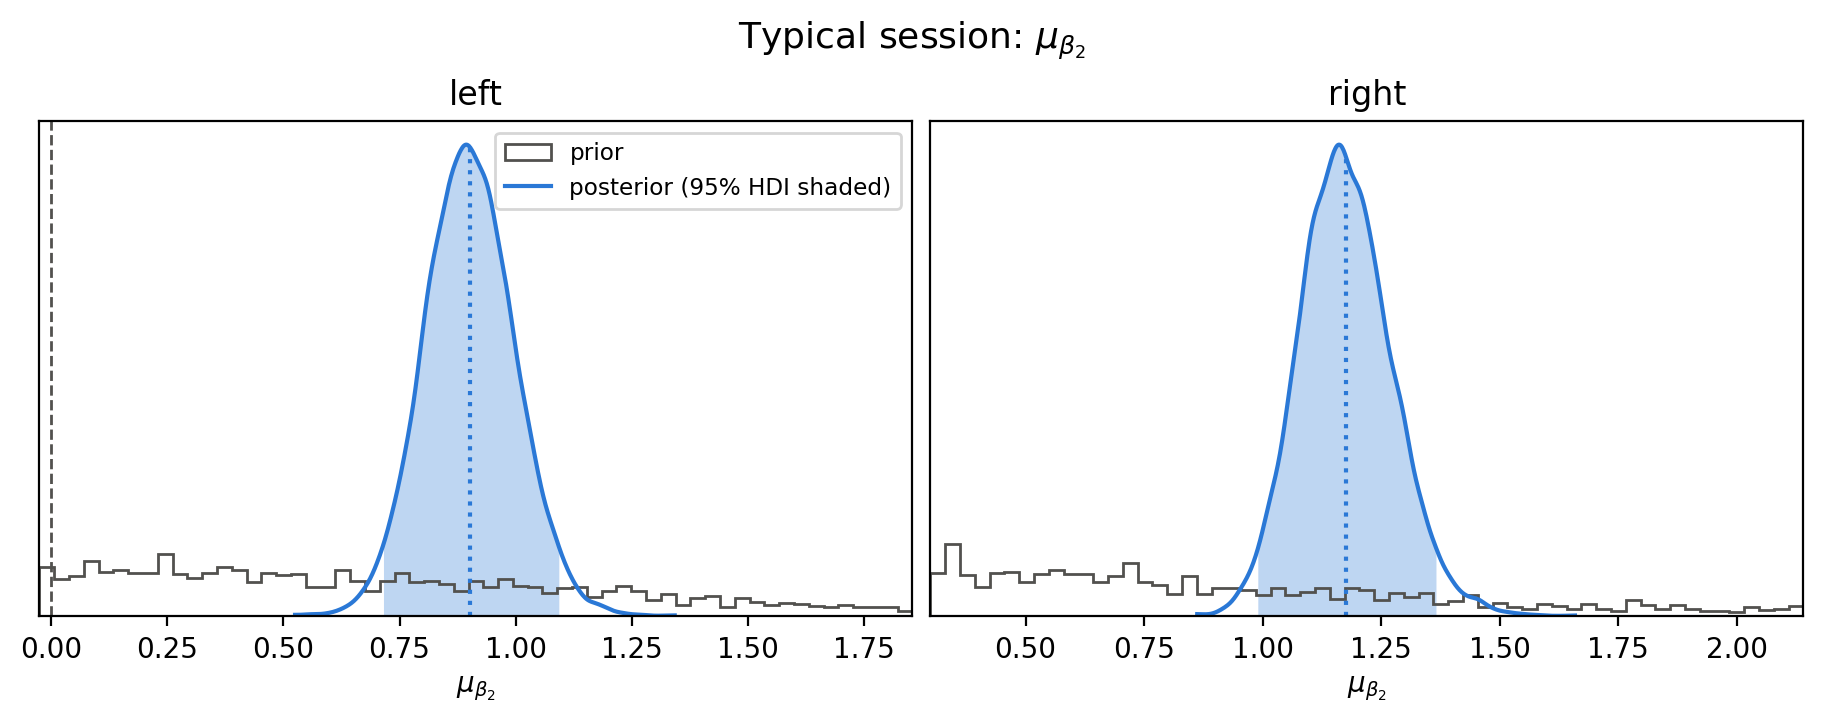
\includegraphics[width=0.8\textwidth]{population_mub2_prior_posterior.png}
\caption{Prior (gray) and posterior (blue) of the hand-level distractor coefficient
$\mu_{\beta_2}$; the dashed line marks 0.}
\label{fig:pop_b2}
\end{figure}

\section{Effect of the Distractor}
\label{sec:effect}

\begin{figure}[H]
\centering
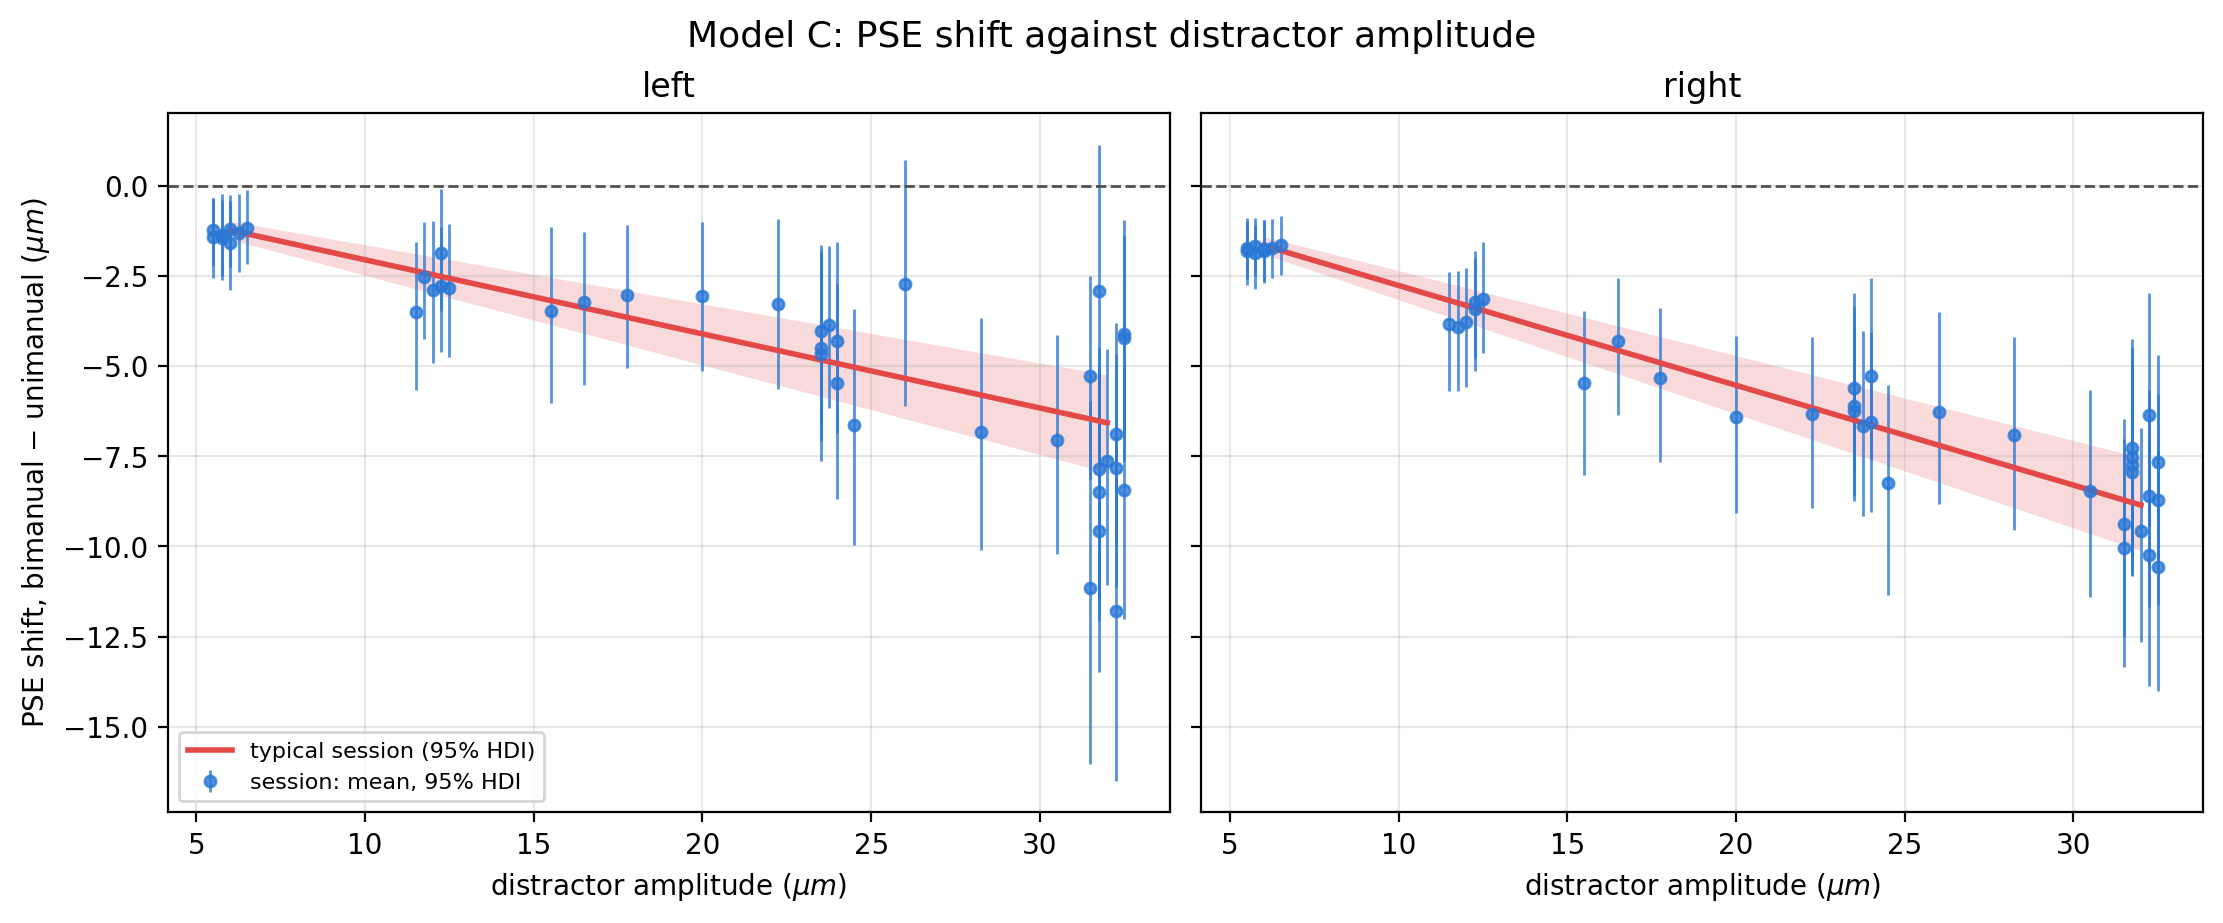
\includegraphics[width=\textwidth]{pse_shift_vs_amplitude.png}
\caption{PSE shift (bimanual $-$ unimanual) against the session's distractor amplitude.
Blue: every session, posterior mean and 95\% HDI (sessions sharing an amplitude are
spread slightly). Red: a typical session, posterior mean and 95\% HDI.}
\label{fig:shift_amp}
\end{figure}

\begin{table}[H]
\centering
\caption{PSE shift (bimanual $-$ unimanual, $\mu m$) of a typical session at the most
used distractor amplitudes: posterior mean [95\% HDI].}
\label{tab:shift}
\begin{tabular}{lcc}
\toprule
distractor ($\mu m$) & left & right \\
\midrule
6  & $-1.23$ [$-1.49$, $-0.98$] & $-1.66$ [$-1.90$, $-1.41$] \\
12 & $-2.46$ [$-2.98$, $-1.97$] & $-3.32$ [$-3.79$, $-2.83$] \\
24 & $-4.93$ [$-5.96$, $-3.93$] & $-6.64$ [$-7.59$, $-5.65$] \\
32 & $-6.57$ [$-7.95$, $-5.24$] & $-8.85$ [$-10.12$, $-7.54$] \\
\bottomrule
\end{tabular}
\end{table}

The distractor lowers the PSE, and by more the stronger it is
(Figure~\ref{fig:shift_amp}, Table~\ref{tab:shift}). The shift is larger for the right
hand at every amplitude. Averaged over the 42 sessions it is $-4.51$ [$-5.15$, $-3.86$]
$\mu m$ for the left hand and $-5.74$ [$-6.39$, $-5.11$] $\mu m$ for the right. At the
session level, the shift's HDI lies below 0 in 40 of 42 sessions (left) and all 42
(right).

The sessions vary only a little around the hand-level line: $\sigma_{\beta_2}$ is 0.30
(left) and 0.23 (right), so the spread of the session shifts in
Figure~\ref{fig:shift_amp} mostly reflects the sessions' different distractor
amplitudes rather than different $\beta_2$. The convergence study showed that a session's $\beta_2$ is
poorly determined when its distractor is weak and is then pulled toward the hand
mean; the 6 $\mu m$ sessions in Figure~\ref{fig:shift_amp} sit almost exactly on the
line.

\subsection{Does the shift scale with amplitude?}
\label{sec:ampcheck}

Model C assumes the shift is proportional to the distractor amplitude. A direct check
needs a measure of the shift that does not depend on the model: for the sessions at
each of the four most used amplitudes, the difference between the proportions of
``high'' responses on bimanual and unimanual trials, over all stimuli. It reflects the
PSE shift and, to a lesser extent, the higher lapse rate $\gamma_h$ on bimanual trials.
Table~\ref{tab:ampcheck} compares the observed difference with its posterior predictive
distribution; Figure~\ref{fig:ampcheck} shows the proportions behind it.

\begin{table}[H]
\centering
\caption{Bimanual $-$ unimanual difference in the proportion of ``high'' responses, in the
sessions at each distractor amplitude: observed, and posterior predictive median and
95\% interval. $P$: posterior predictive probability of a difference below the
observed one.}
\label{tab:ampcheck}
\begin{tabular}{llccccc}
\toprule
hand & distractor & sessions & observed & predicted & 95\% interval & $P$ \\
\midrule
left  & 6 $\mu m$  & 8  & 0.011 & 0.035 & [0.002, 0.068] & 0.07 \\
left  & 12 $\mu m$ & 6  & 0.081 & 0.050 & [0.014, 0.087] & 0.95 \\
left  & 24 $\mu m$ & 7  & 0.092 & 0.082 & [0.046, 0.119] & 0.71 \\
left  & 32 $\mu m$ & 13 & 0.148 & 0.131 & [0.099, 0.164] & 0.85 \\
right & 6 $\mu m$  & 8  & 0.073 & 0.040 & [0.009, 0.071] & 0.98 \\
right & 12 $\mu m$ & 6  & 0.088 & 0.063 & [0.027, 0.103] & 0.90 \\
right & 24 $\mu m$ & 7  & 0.113 & 0.114 & [0.076, 0.151] & 0.49 \\
right & 32 $\mu m$ & 13 & 0.161 & 0.153 & [0.122, 0.184] & 0.69 \\
\bottomrule
\end{tabular}
\end{table}

\begin{figure}[H]
\centering
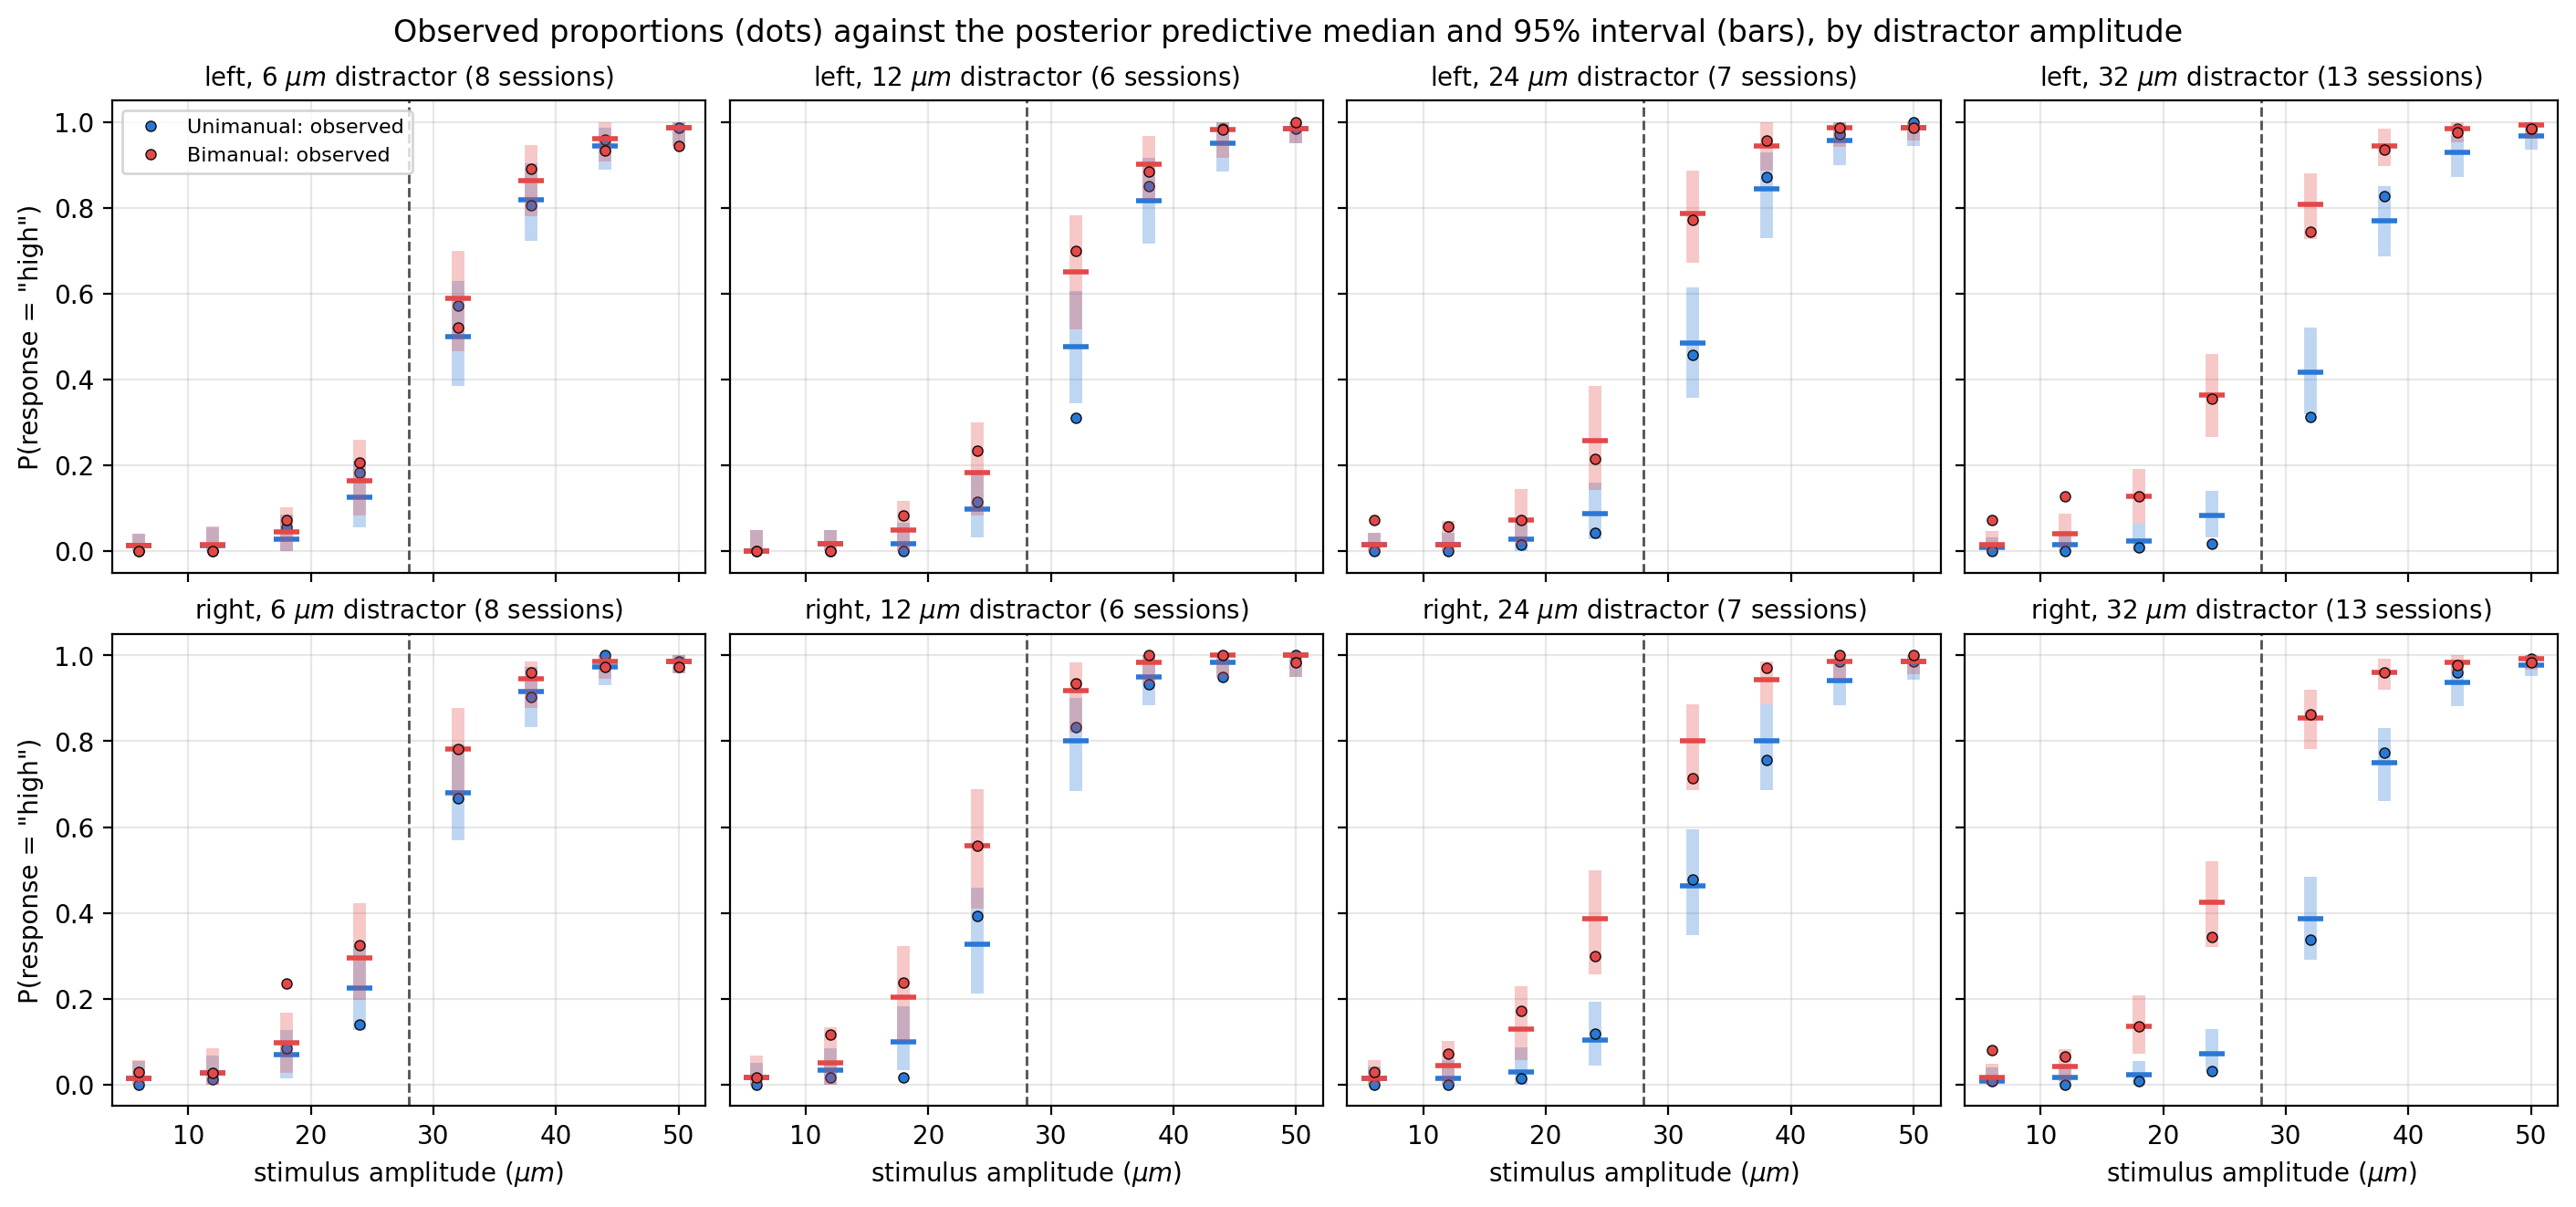
\includegraphics[width=\textwidth]{ppc_by_distractor_amplitude.png}
\caption{Observed proportions of ``high'' responses (dots) against the posterior
predictive median and 95\% interval (bars), in the sessions at each distractor
amplitude. Unimanual in blue, bimanual in red.}
\label{fig:ampcheck}
\end{figure}

Seven of the eight observed differences lie inside their predictive intervals. The
exception is the right hand at 6 $\mu m$: the observed difference, 0.073, lies above the
interval [0.009, 0.071], and the model predicts a smaller difference in 98\% of its
replicates. In Figure~\ref{fig:ampcheck} this shows at 18 $\mu m$, where the right-hand
bimanual proportion lies well above its predicted range. For the right hand, then, even a
weak distractor shifts responses more than a proportional model allows, the presence
effect suggested by the comparison with Model B. The left hand at 6 $\mu m$ goes the
other way: its observed difference is smaller than predicted ($P = 0.07$), so for the
left hand a proportional shift is, if anything, too large at weak distractors.

\begin{figure}[H]
\centering
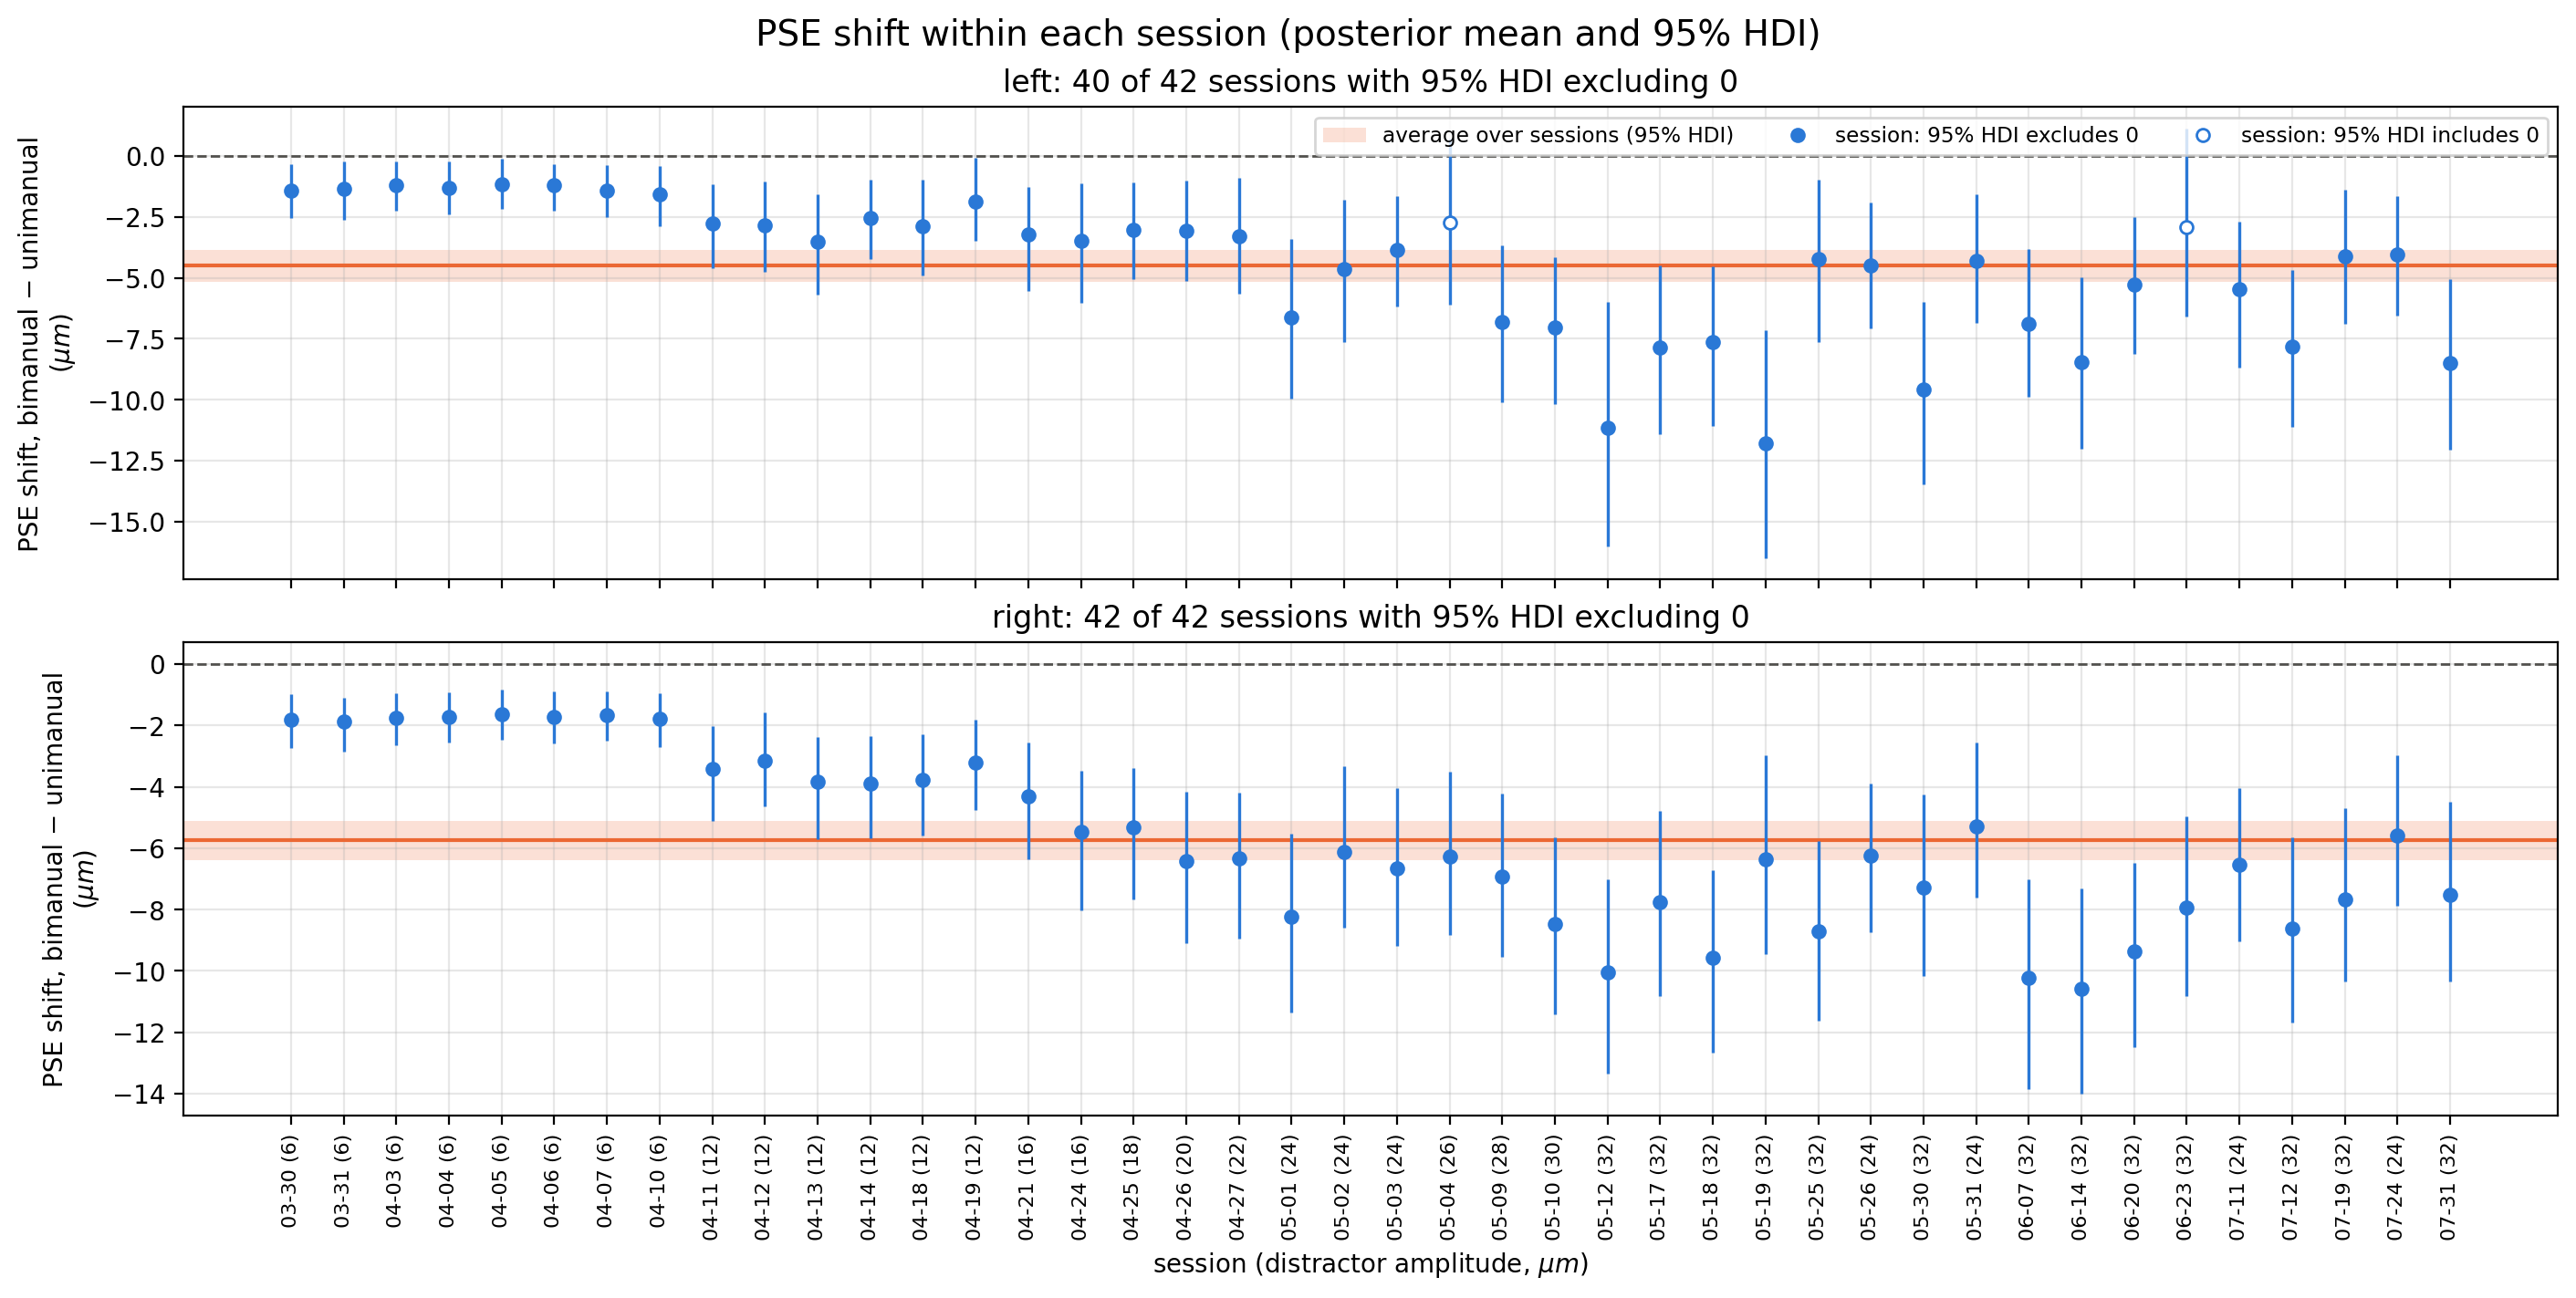
\includegraphics[width=\textwidth]{effect_PSE_by_session.png}
\caption{PSE shift (bimanual $-$ unimanual) within each session, in date order with
the distractor amplitude in brackets: posterior mean and 95\% HDI (filled: HDI
excludes 0). The orange band is the average over the 42 sessions.}
\label{fig:shift_sess}
\end{figure}

In date order (Figure~\ref{fig:shift_sess}) the session shifts follow the
amplitude schedule: small in the first eight sessions, which all used 6 $\mu m$,
and largest in the 32 $\mu m$ sessions from May onwards.

By construction, Model C cannot show an effect of the distractor on the JND or the
lapse rates.

\subsection{Session estimates}

\begin{figure}[H]
\centering
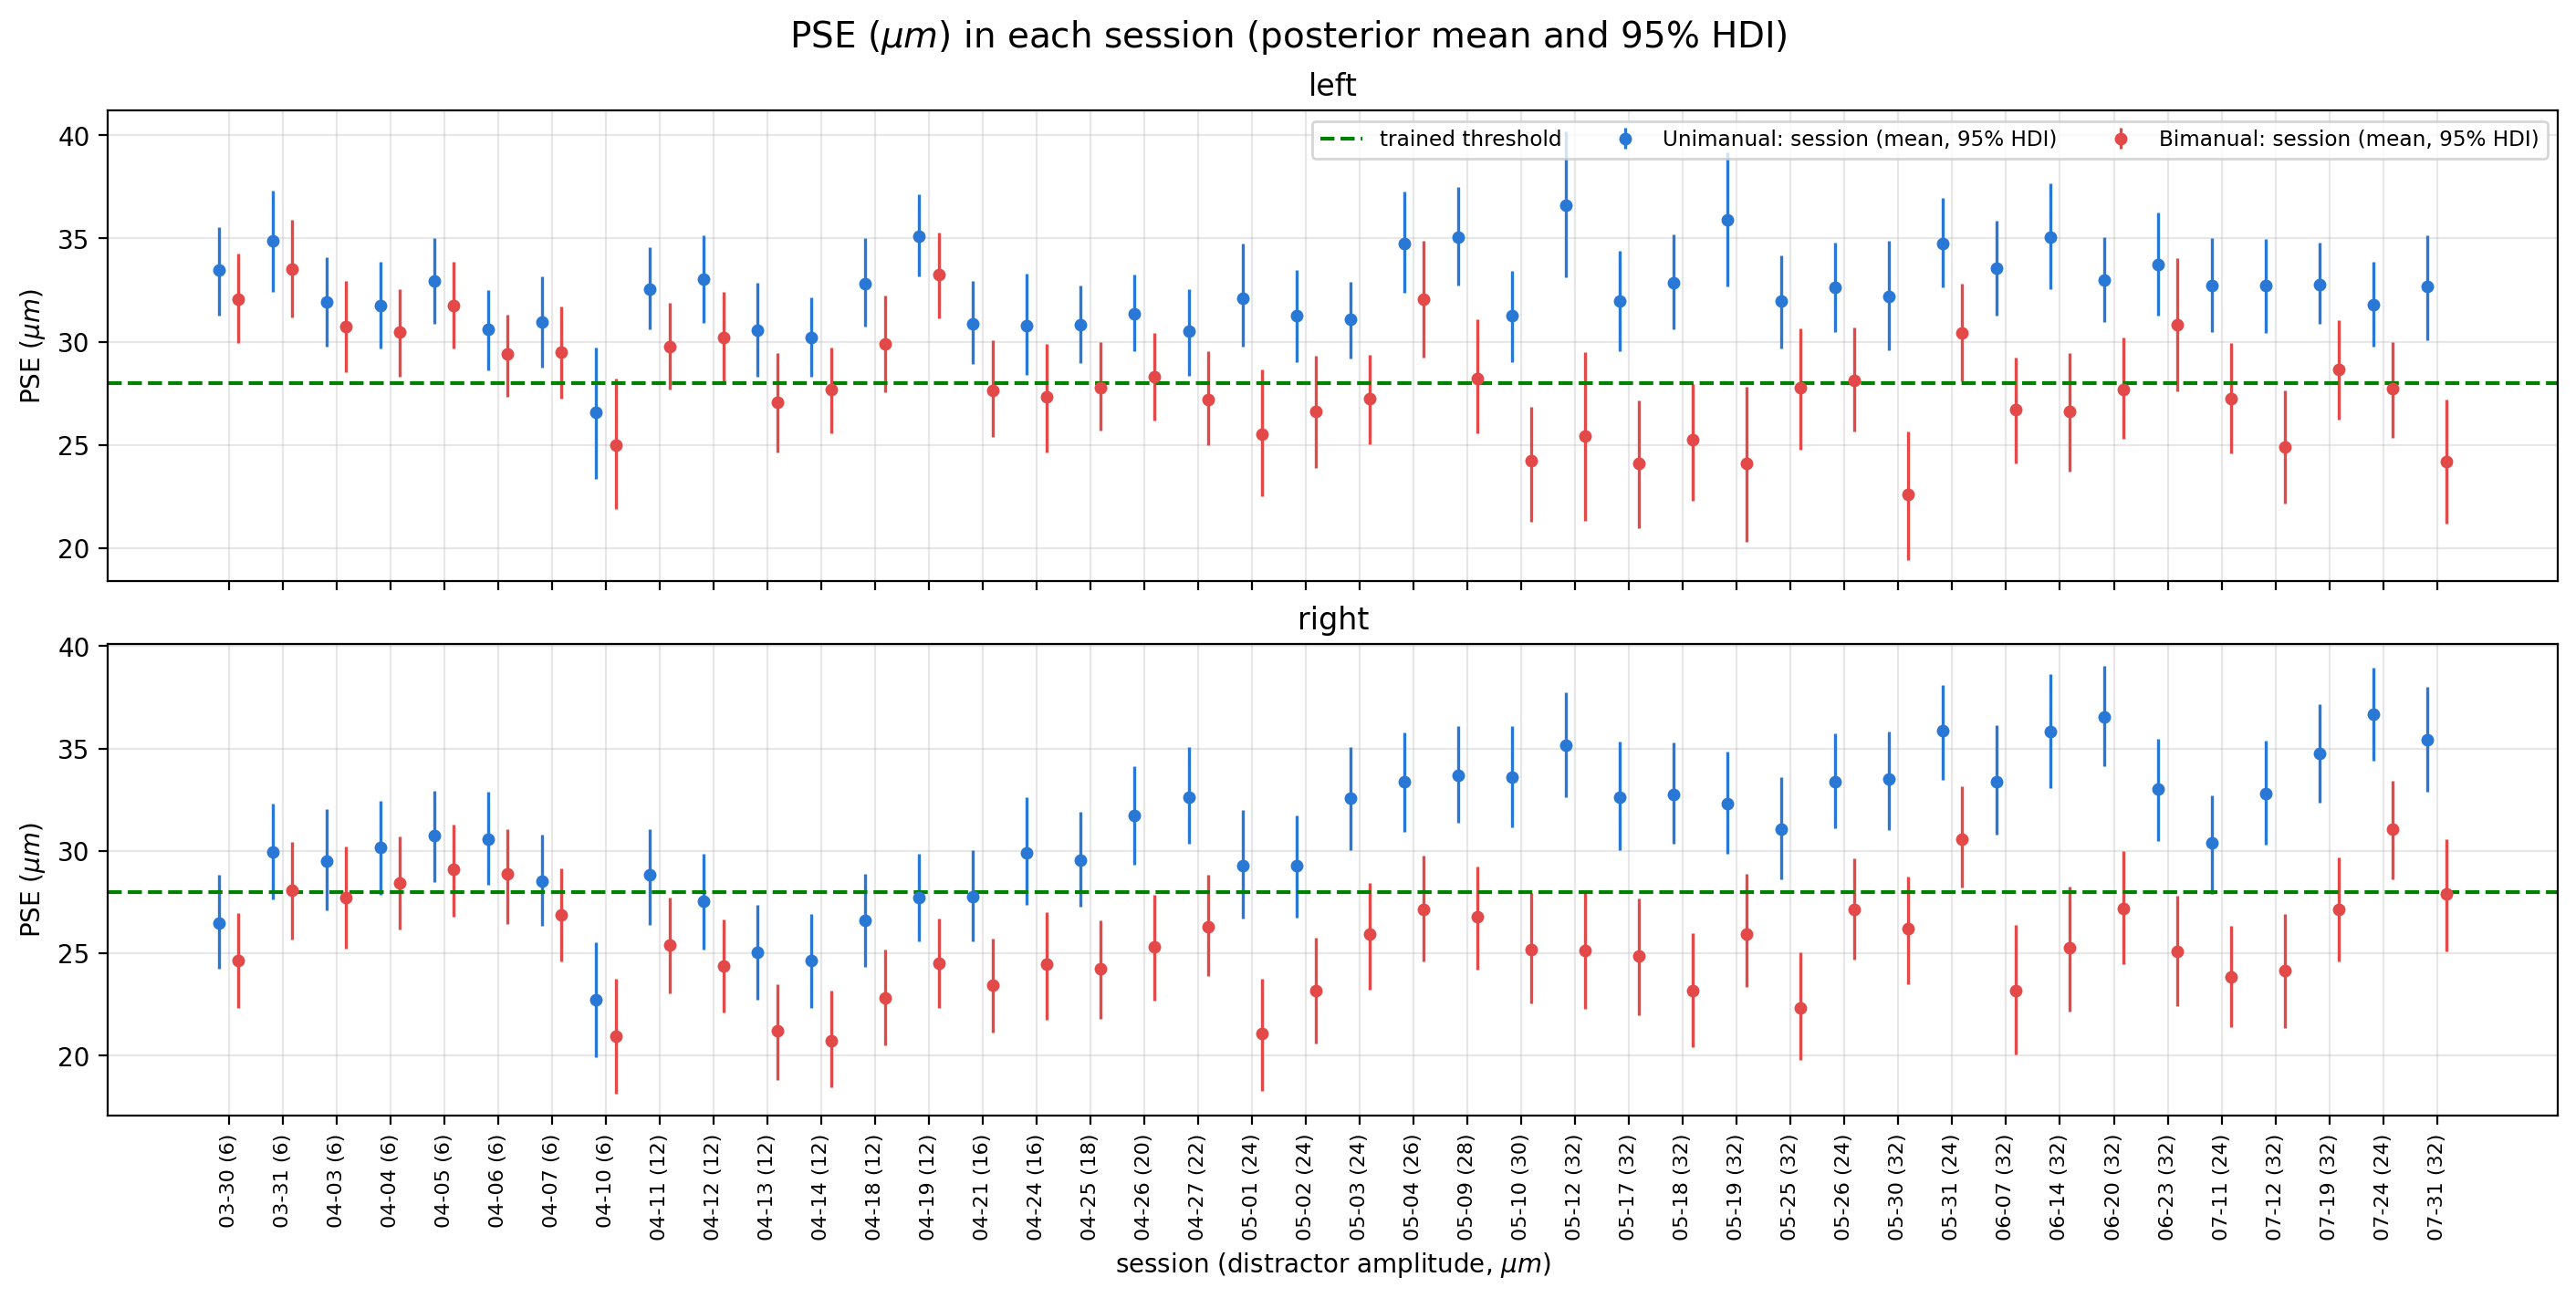
\includegraphics[width=\textwidth]{PSE_by_session.png}
\caption{Unimanual (blue) and bimanual (red) PSE in each session: posterior mean
and 95\% HDI. The dashed line is the trained threshold.}
\label{fig:pse_sess}
\end{figure}

The session PSEs range from 26.6 to 36.6 $\mu m$ (left) and 22.7 to 36.7 $\mu m$
(right) on unimanual trials, and from 22.6 to 33.5 and 20.7 to 31.1 $\mu m$ on
bimanual trials (Figure~\ref{fig:pse_sess}). Both conditions move together from
session to session, which the within-session shift cancels.

\begin{figure}[H]
\centering
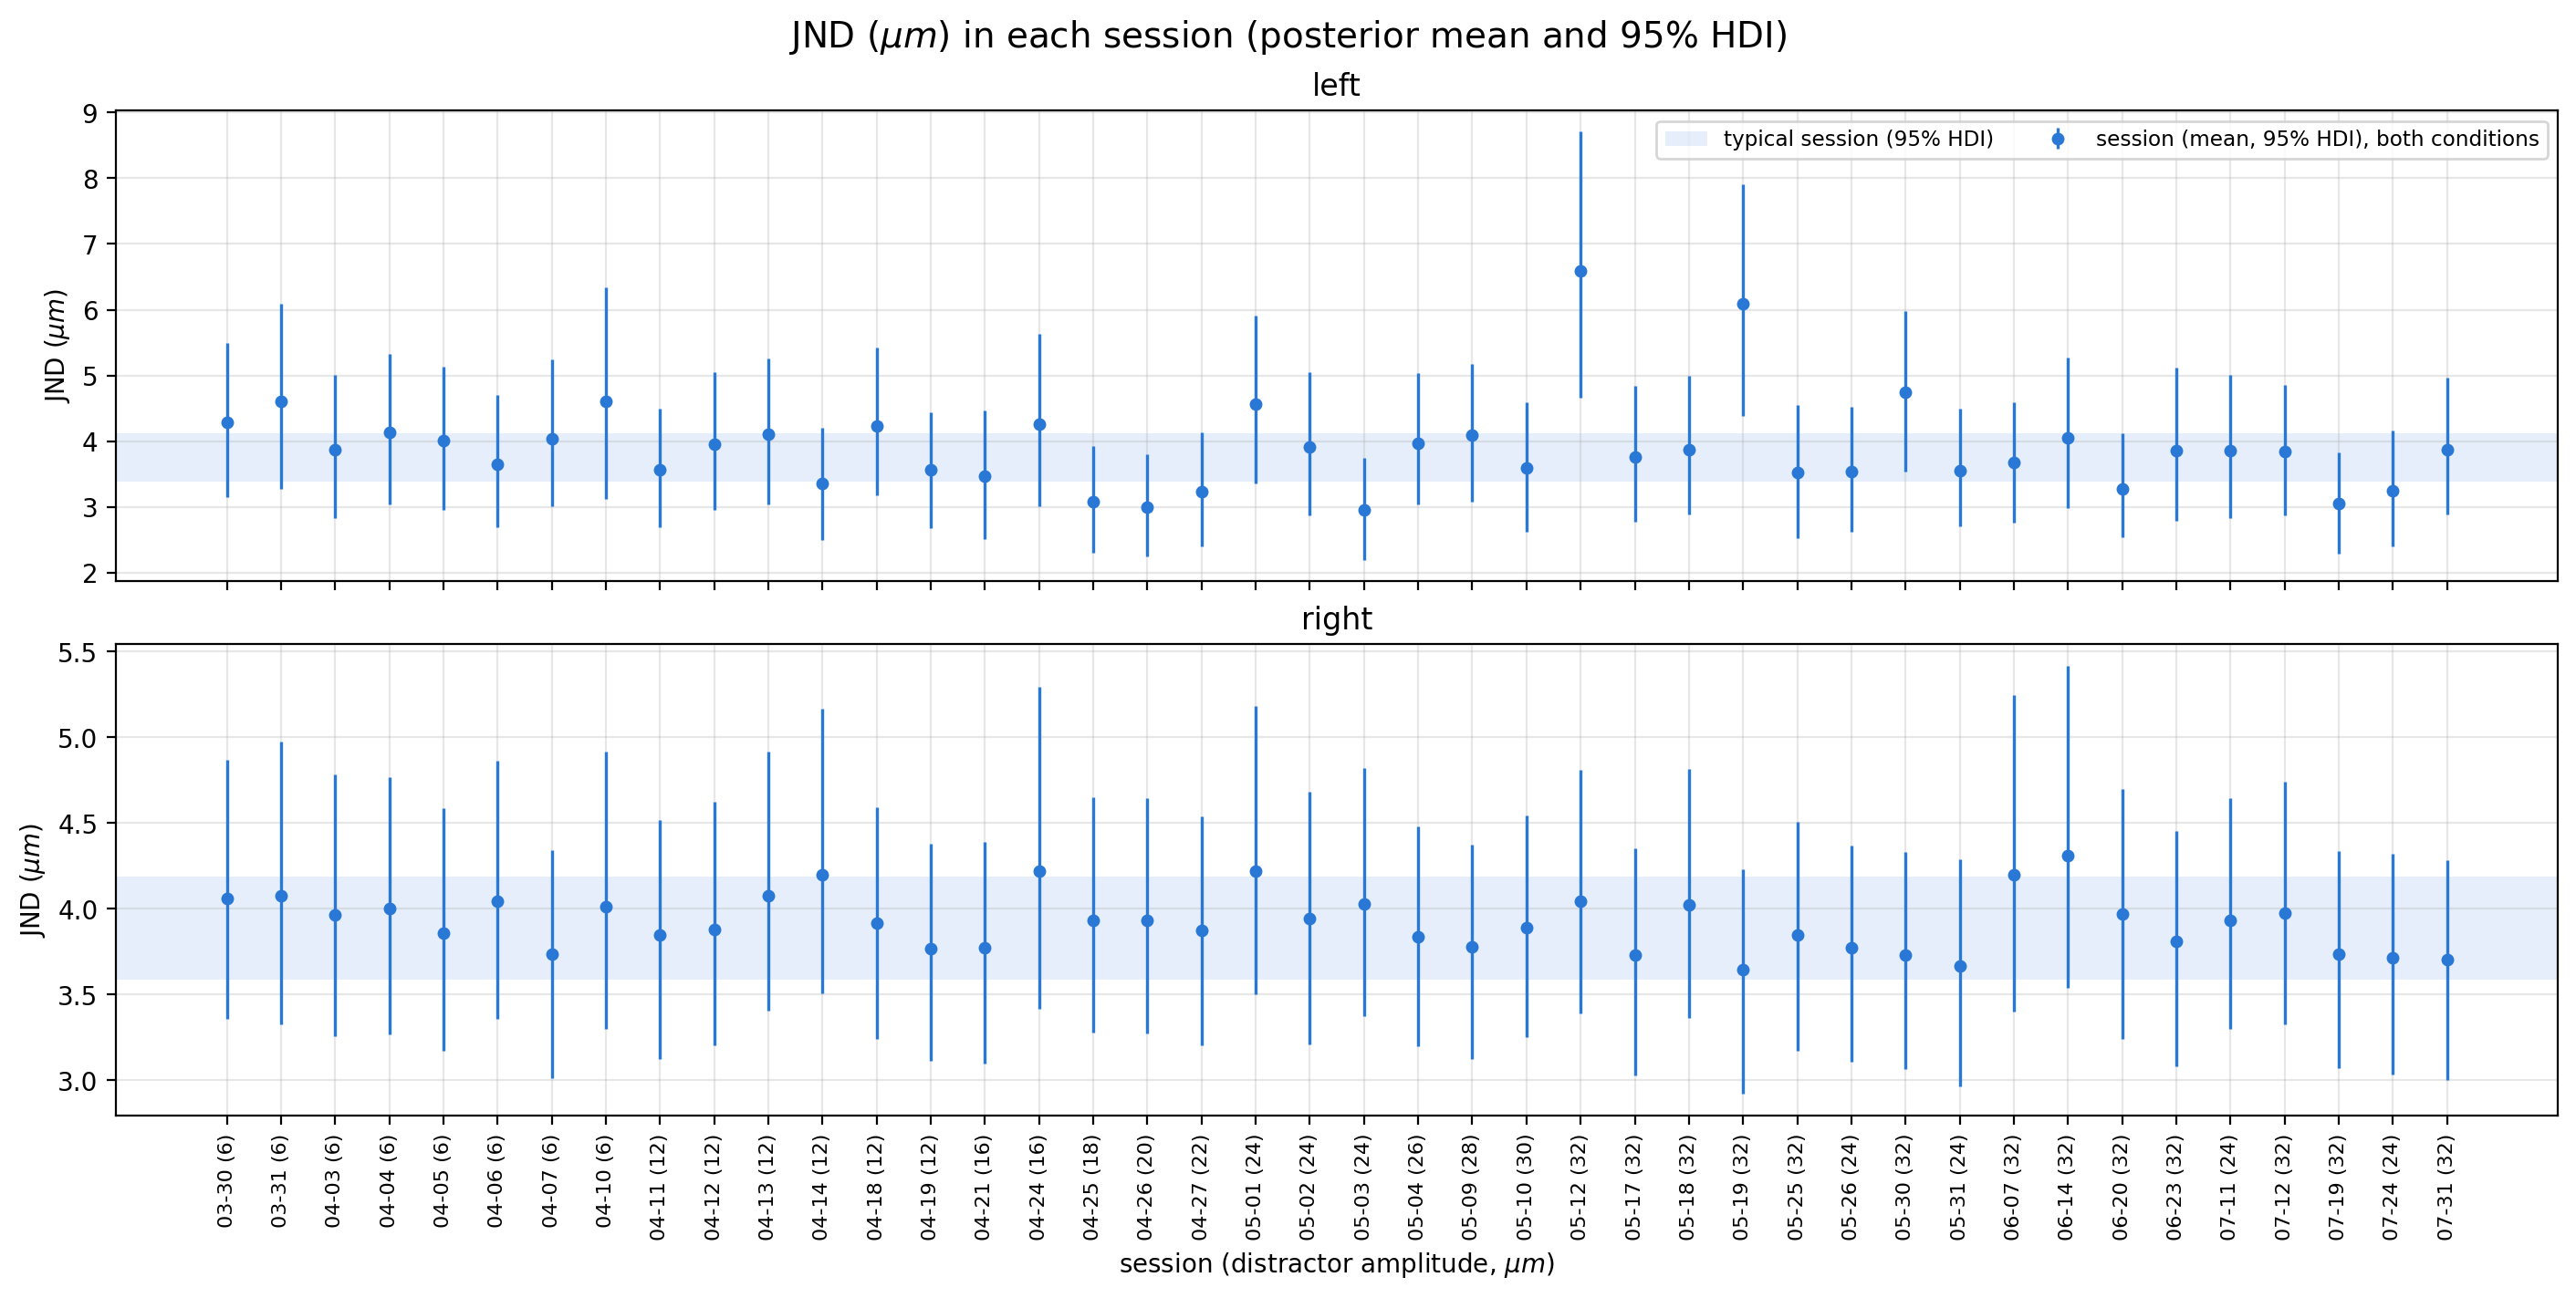
\includegraphics[width=\textwidth]{JND_by_session.png}
\caption{JND in each session, shared by both conditions: posterior mean and 95\% HDI.
The band is a typical session's 95\% HDI.}
\label{fig:jnd_sess}
\end{figure}

\begin{figure}[H]
\centering
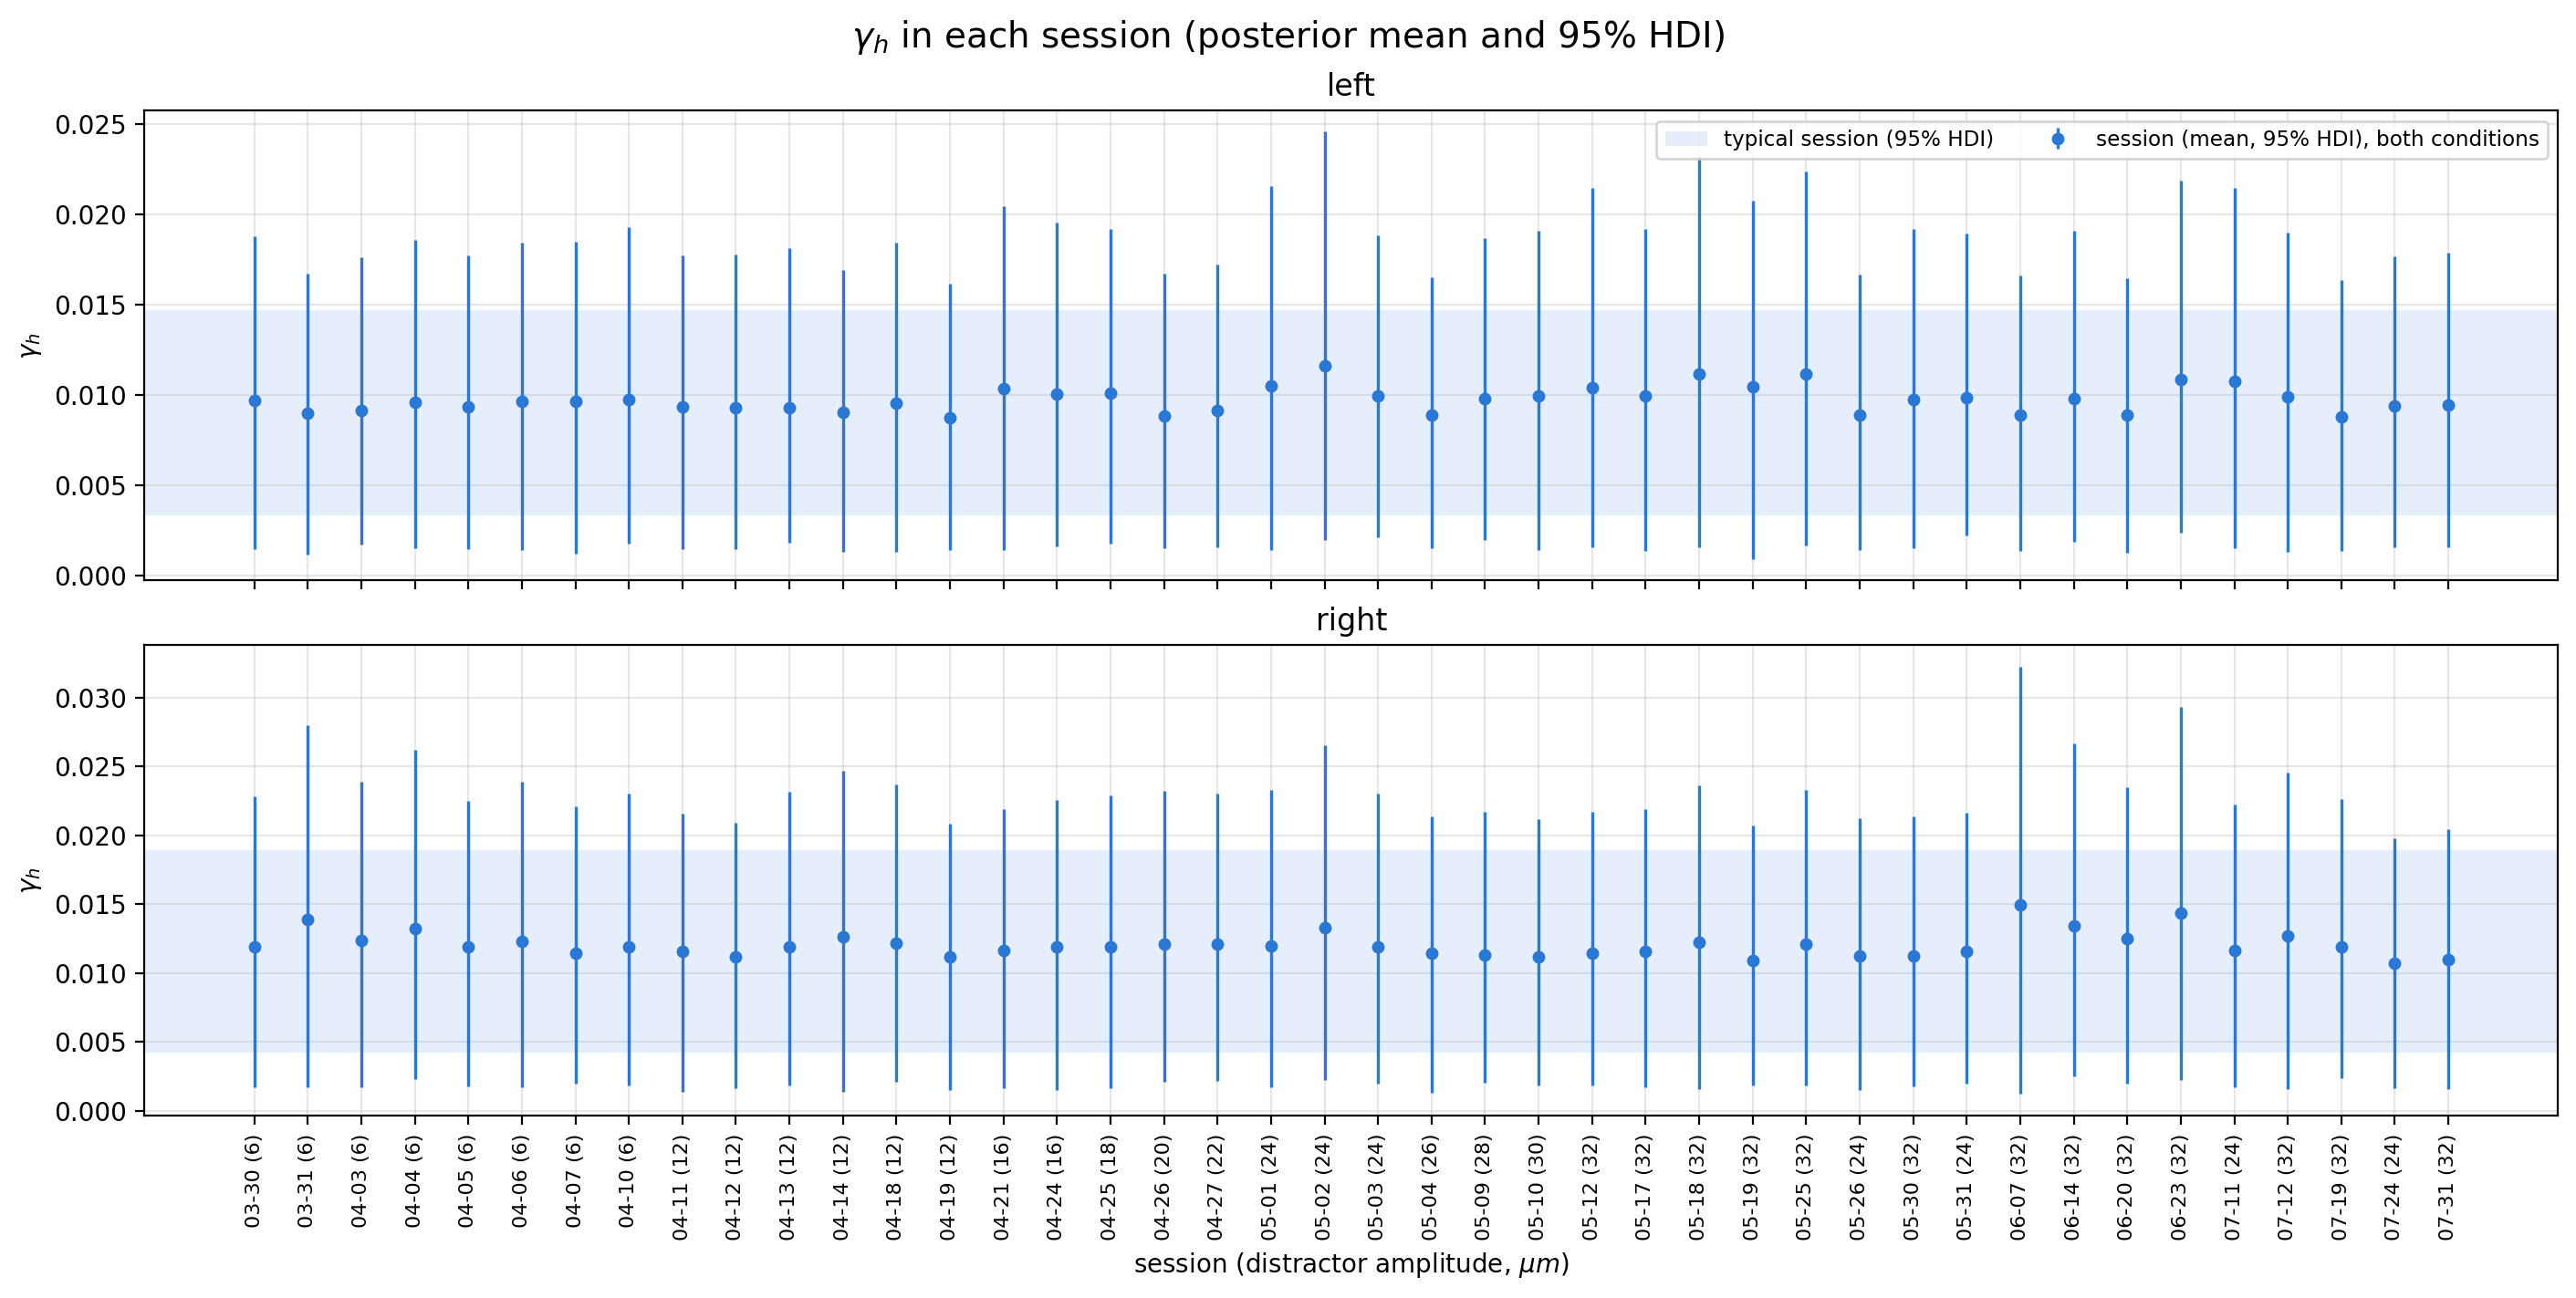
\includegraphics[width=\textwidth]{gamh_by_session.png}
\caption{$\gamma_h$ in each session, shared by both conditions.}
\label{fig:gamh_sess}
\end{figure}

\begin{figure}[H]
\centering
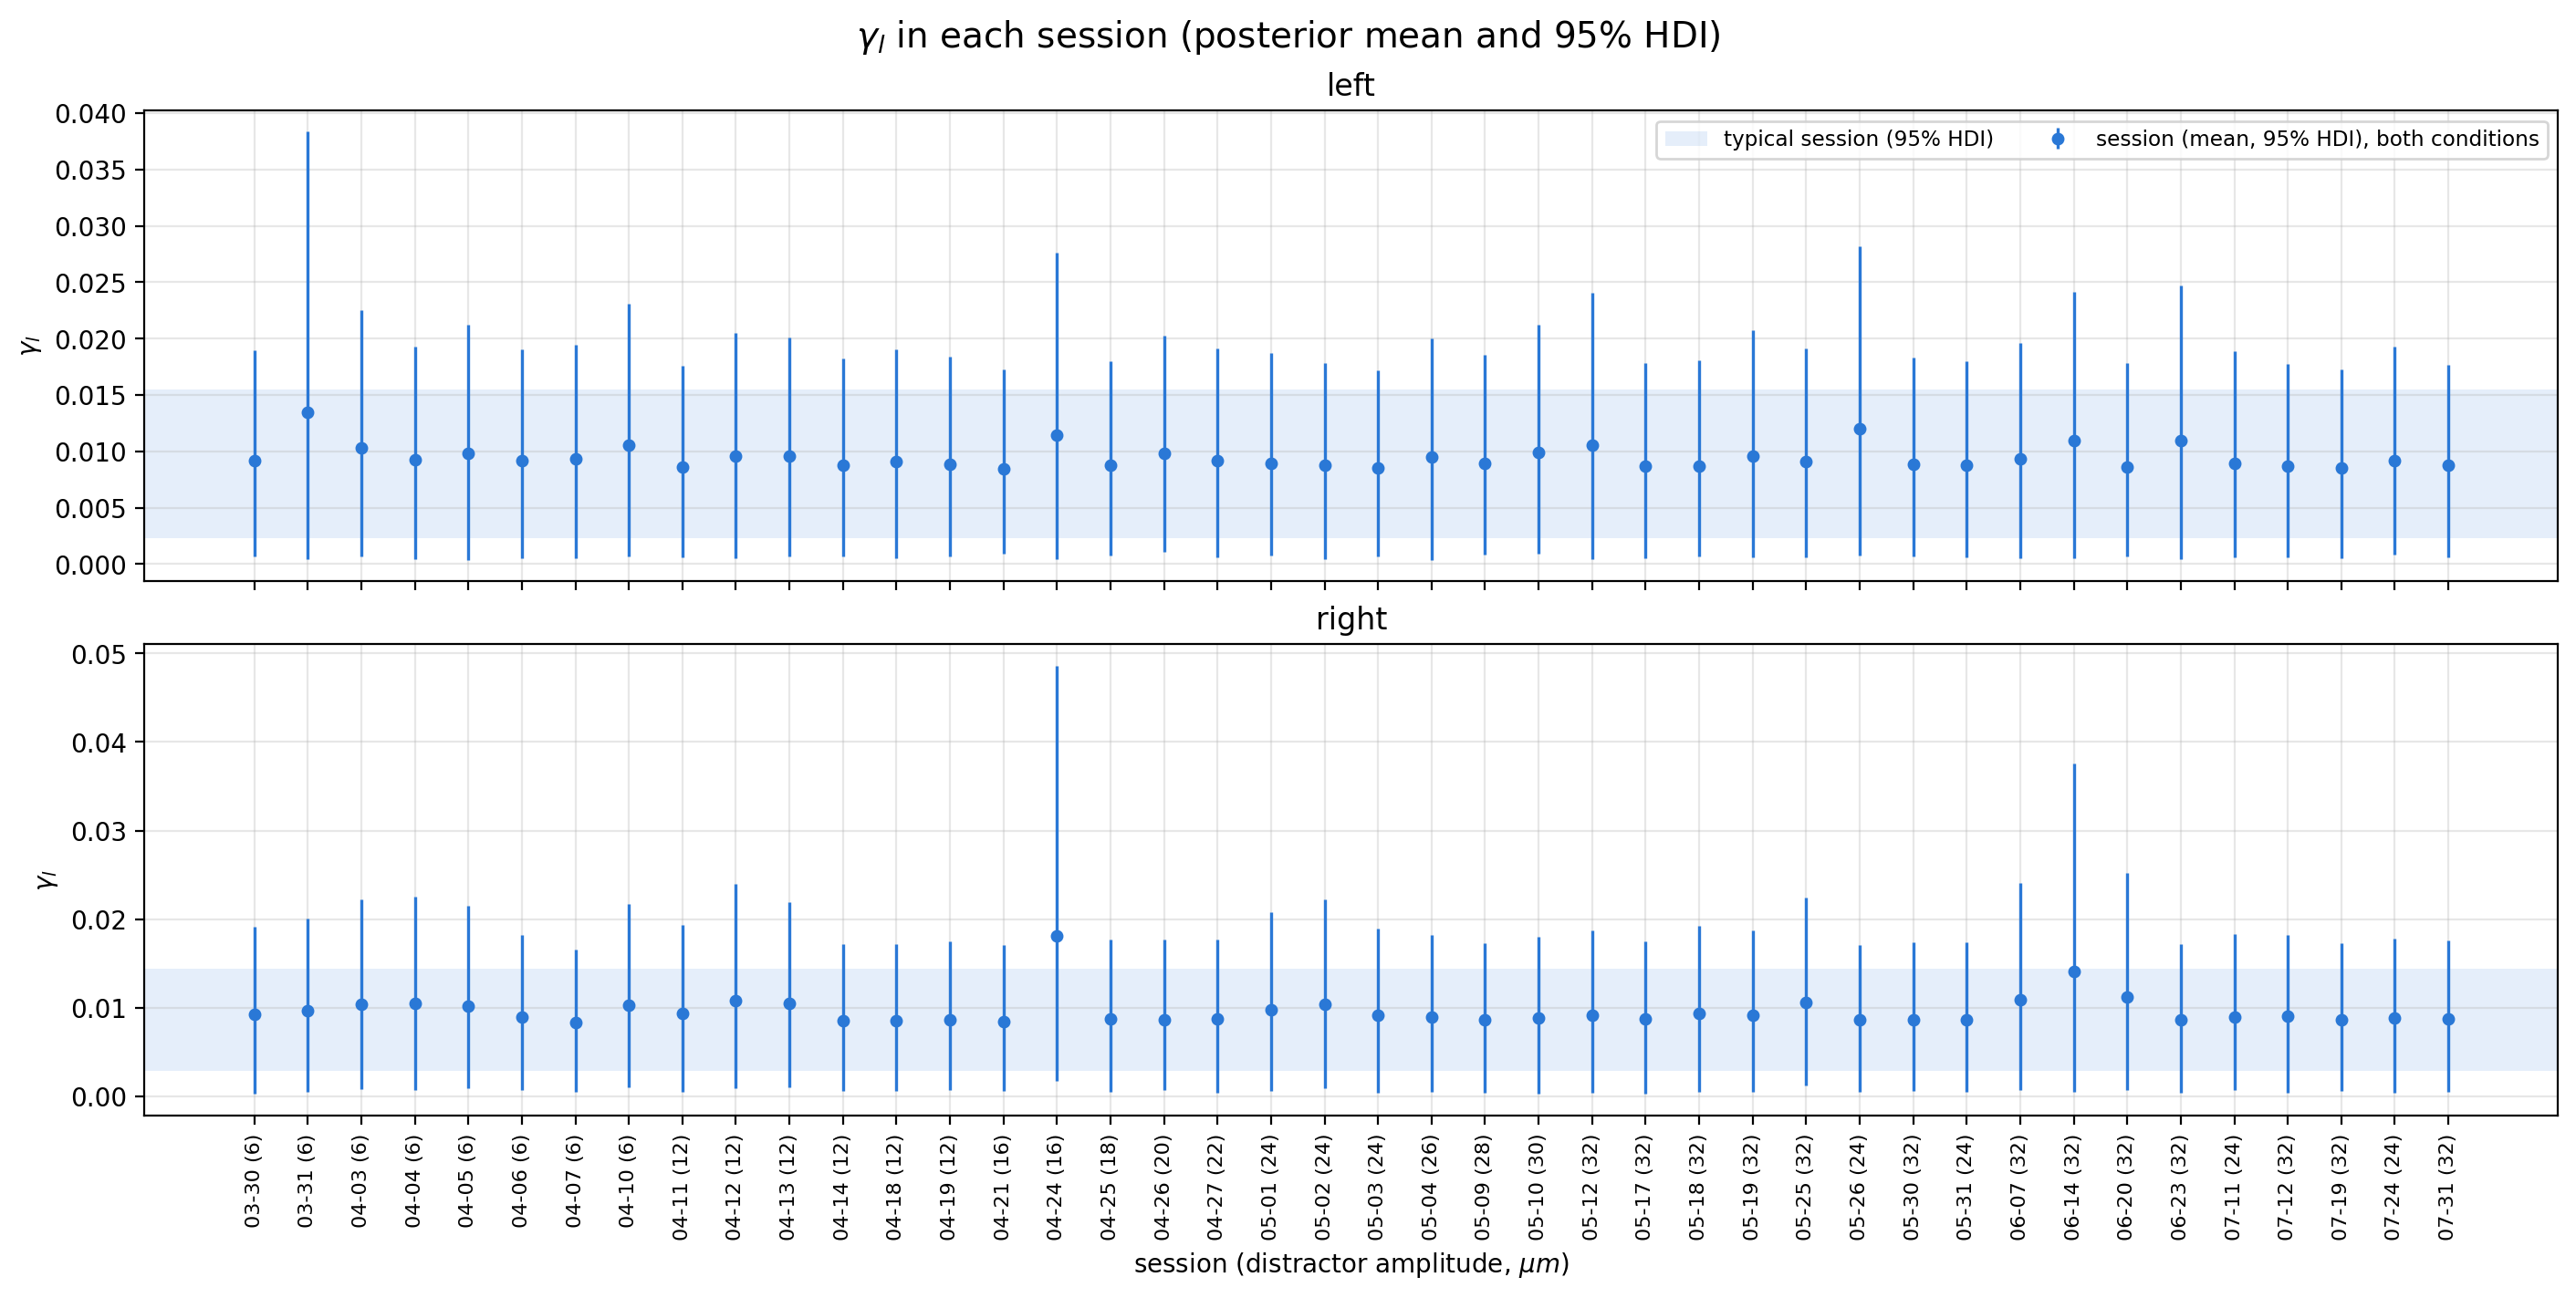
\includegraphics[width=\textwidth]{gaml_by_session.png}
\caption{$\gamma_l$ in each session, shared by both conditions.}
\label{fig:gaml_sess}
\end{figure}

The left-hand JNDs vary between sessions ($\sigma_{\beta_1} = 0.90$), from 2.95 to
6.59 $\mu m$, with the two shallowest sessions in mid-May; the right-hand ones barely
vary, from 3.65 to 4.31 $\mu m$ (Figure~\ref{fig:jnd_sess}). The session lapse rates
are almost identical within a hand (Figures~\ref{fig:gamh_sess}
and~\ref{fig:gaml_sess}): the posterior means of $\gamma_h$ range only from 0.0087 to
0.0116 (left) and 0.0107 to 0.0149 (right). With $\sigma_{\gamma_h}$ and
$\sigma_{\gamma_l}$ not identified, every session is pulled to its hand's typical
value, so these plots say little about real day-to-day differences in lapses.

\section{Comparison with Model B}

Model B fits unimanual and bimanual trials as separate groups, each with its own
per-session parameters, and has no amplitude covariate. Both models were fit to the
same trials in the same order.

\paragraph{Leave-one-out cross-validation.}
Model C has $\text{elpd}_\text{loo} = -3217.0$ (SE 65.7) with $p_\text{loo} = 138.6$ and
every Pareto $k$ at most 0.33; Model B has $-3180.0$ (SE 64.3) with
$p_\text{loo} = 178.7$. Model C is worse by 37.1 (SE 11.9), 3.1 standard errors,
despite needing fewer effective parameters.

\begin{table}[H]
\centering
\caption{$\text{elpd}_\text{loo}(\text{C}) - \text{elpd}_\text{loo}(\text{B})$ summed over the
trials at each amplitude, by hand and condition. Negative values favor Model B.}
\label{tab:loo}
\begin{tabular}{rcccc}
\toprule
 & \multicolumn{2}{c}{left} & \multicolumn{2}{c}{right} \\
amplitude ($\mu m$) & bimanual & unimanual & bimanual & unimanual \\
\midrule
6  & $-6.6$ & $-3.5$ & $-5.1$ & $-2.3$ \\
12 & $-4.2$ & $-3.0$ & $-1.8$ & $-2.8$ \\
18 & 0.7 & $-1.6$ & $-3.4$ & $-0.3$ \\
24 & $-1.0$ & 0.8 & 1.9 & 0.8 \\
32 & $-0.1$ & $-3.4$ & 0.3 & 1.7 \\
38 & $-0.3$ & $-1.4$ & 0.2 & 1.6 \\
44 & 0.0 & $-3.8$ & 0.4 & $-1.5$ \\
50 & $-0.1$ & 0.3 & 0.1 & 0.0 \\
\bottomrule
\end{tabular}
\end{table}

Model C loses 29.2 of its 37.1 at the 6 and 12 $\mu m$ stimuli (Table~\ref{tab:loo}):
17.6 on bimanual and 11.6 on unimanual trials. This is the shared-lapse misfit of
Section~\ref{sec:ppc}, seen from both sides. The next largest losses are on left
unimanual trials at 32 and 44 $\mu m$ ($-3.4$ and $-3.8$), on the rising part of the
curve. With one slope for both conditions, Model C cannot give the left-hand unimanual
curve a different steepness than the bimanual one, which Model B allows.

\paragraph{Session PSE shifts.}

\begin{figure}[H]
\centering
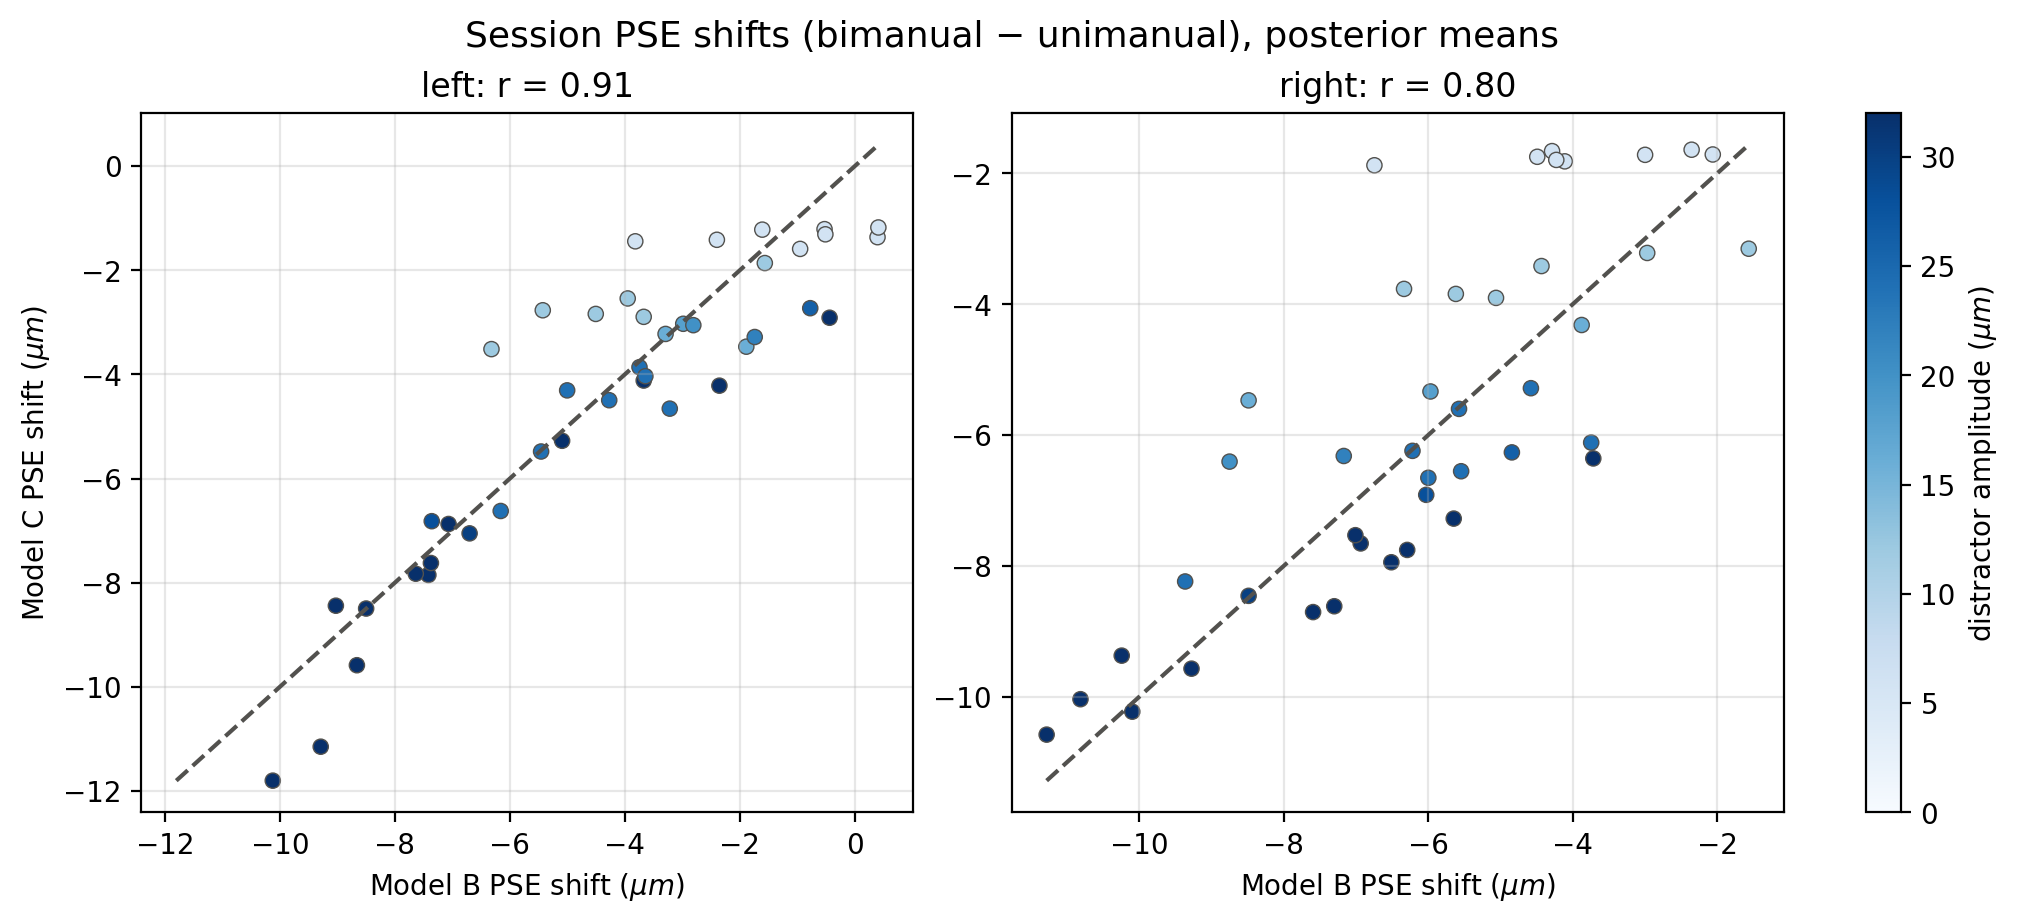
\includegraphics[width=\textwidth]{pse_shift_C_vs_B.png}
\caption{Session PSE shifts (bimanual $-$ unimanual), posterior means: Model C
against Model B, colored by the session's distractor amplitude. The dashed line is the
identity; $r$ is the correlation.}
\label{fig:CvsB}
\end{figure}

The two models agree on the average shift ($-4.51$ against $-4.29$ $\mu m$ for the left
hand, $-5.74$ against $-6.06$ for the right) and, for the left hand, closely on the
session shifts ($r = 0.91$, Figure~\ref{fig:CvsB}). For the right hand ($r = 0.80$) they
disagree at the weakest distractor:

\begin{table}[H]
\centering
\caption{Session PSE shifts ($\mu m$) at the weakest and strongest distractor: mean and
range of the posterior means over the sessions with that amplitude.}
\label{tab:small}
\begin{tabular}{llcc}
\toprule
hand & distractor & Model B & Model C \\
\midrule
left  & 6 $\mu m$ (8 sessions)  & $-1.13$ ($-3.82$ to 0.41) & $-1.34$ ($-1.59$ to $-1.18$) \\
left  & 32 $\mu m$ (13 sessions) & $-6.67$ ($-10.12$ to $-0.44$) & $-7.40$ ($-11.80$ to $-2.91$) \\
right & 6 $\mu m$ (8 sessions)  & $-3.91$ ($-6.74$ to $-2.06$) & $-1.75$ ($-1.88$ to $-1.64$) \\
right & 32 $\mu m$ (13 sessions) & $-7.90$ ($-11.28$ to $-3.72$) & $-8.58$ ($-10.58$ to $-6.36$) \\
\bottomrule
\end{tabular}
\end{table}

For the right hand, Model B estimates the 6 $\mu m$ sessions to shift by 3.91 $\mu m$ on
average, Model C by only 1.75 (Table~\ref{tab:small}). Model C's shift is proportional
to the amplitude, so a weak distractor must give a small shift, and with $\beta_2$
poorly determined in these sessions they all fall onto the hand-level line. Model B,
which estimates each session's shift freely, suggests that for the right hand even a
weak distractor shifts the PSE substantially: an effect of the distractor being
present, on top of its amplitude.

\section{Conclusions}
\label{sec:conclusions}

\begin{itemize}
  \item The fit is reliable: 2 divergences in 20{,}000 draws, $\hat{R} = 1.000$ and
        bulk ESS $\ge 3{,}410$ for every variable, every Pareto $k$ good.
  \item The PSE shift grows with distractor amplitude for both hands
        ($\mu_{\beta_2} > 0$ with posterior probability 1.000), more steeply for the
        right hand. This is the main new result of Model C, and it supports the
        exploratory amplitude trend in the Model B report.
  \item Model C predicts the data worse than Model B (elpd difference $-37.1$,
        SE 11.9). The misfit sits where three of its assumptions meet the data:
        \begin{enumerate}
          \item one lapse rate for both conditions, while the distractor raises
                $\gamma_h$: too few ``high'' responses are predicted at weak stimuli on
                bimanual trials, and too many on unimanual ones;
          \item one slope for both conditions, which costs fit on the rising part of
                the left-hand unimanual curve;
          \item a shift proportional to amplitude: for the right hand at 6 $\mu m$,
                Model C's shift is less than half of Model B's, and the observed
                bimanual $-$ unimanual difference lies outside Model C's predictive
                interval (Section~\ref{sec:ampcheck}).
        \end{enumerate}
  \item The size of the shift at weak distractors, and Model C's lapse rates and JNDs,
        should therefore not be taken at face value until these assumptions are
        relaxed.
\end{itemize}

\paragraph{Recommended revisions.}
\begin{enumerate}
  \item Lapse rates per hand and condition (unimanual, bimanual). The evidence for this
        is the strongest.
  \item A distractor-presence term, $\beta_3 \cdot \mathbb{1}[\text{bimanual}]$, so that
        the PSE shift is $-(\beta_3 + \beta_2 d)/\beta_1$ rather than proportional to
        $d$.
  \item Possibly a separate slope on bimanual trials, which would let the distractor
        change the JND.
\end{enumerate}
Each revision changes the model, so it would need a new convergence study before
being fit to the real data again.

\appendix
\section{Joint Posteriors}
\label{app:pairs}

\code{Main\_Analysis\_C.py} also plots joint posteriors for session 04-13
(Figures~\ref{fig:pair_left}--\ref{fig:pair_hyper}). The new parameter $\beta_2$ is
negatively correlated with $\beta_0$ ($r = -0.35$ left, $-0.25$ right): a session's
bimanual position is $\beta_0 + \beta_2 d_s$, so a higher bias can be traded for a
smaller distractor effect, but the unimanual trials pin down $\beta_0$ well enough to
keep the correlation moderate. All other correlations between the session parameters
are at most 0.32 in absolute value (that of $\beta_0$ and $\beta_1$ for the right
hand). There is no ridge or multimodality that would indicate an identifiability
problem.

The left hand's $\gamma_h$ on 04-13 is correlated with its hyperparameter
$\mu_{\gamma_h}$ ($r = 0.60$) but hardly with $\sigma_{\gamma_h}$ ($r = -0.09$)
(Figure~\ref{fig:pair_hyper}): with $\sigma_{\gamma_h}$ small, the session value
follows the hand's typical value.

\begin{figure}[H]
\centering
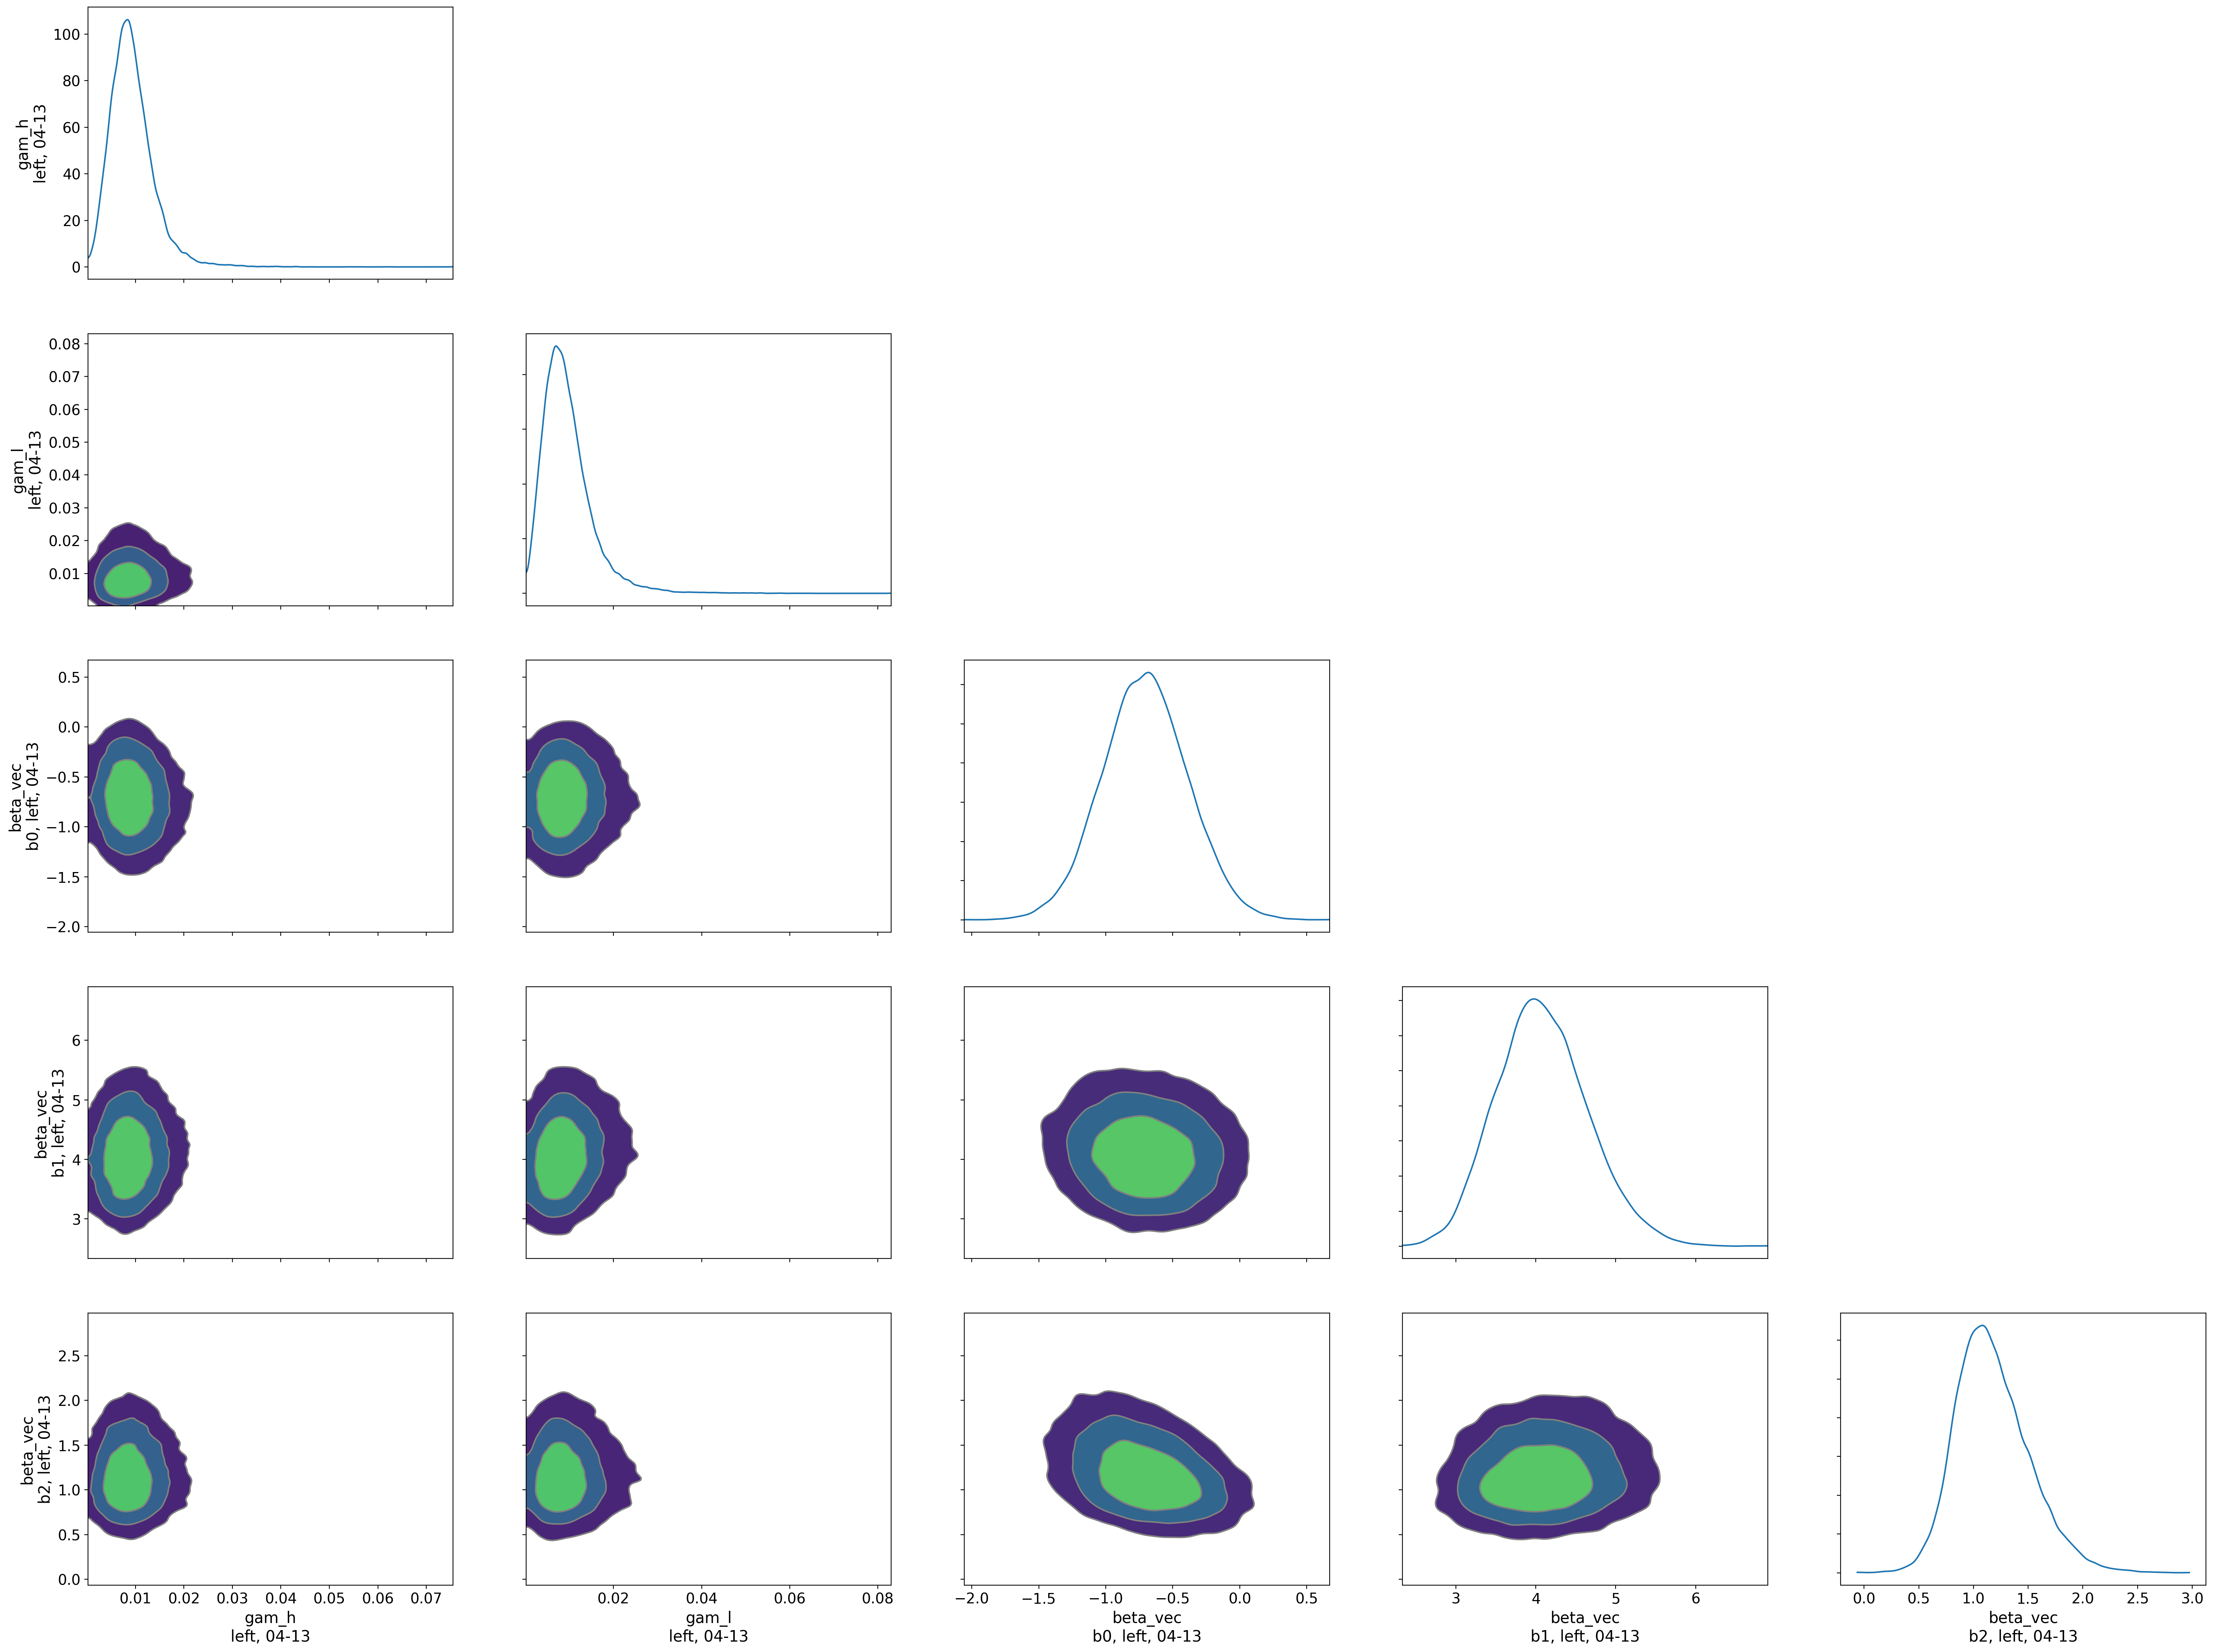
\includegraphics[width=0.85\textwidth]{pair_left_04-13.png}
\caption{Joint posterior of $\gamma_h$, $\gamma_l$, $\beta_0$, $\beta_1$ and $\beta_2$
for the left hand, session 04-13.}
\label{fig:pair_left}
\end{figure}

\begin{figure}[H]
\centering
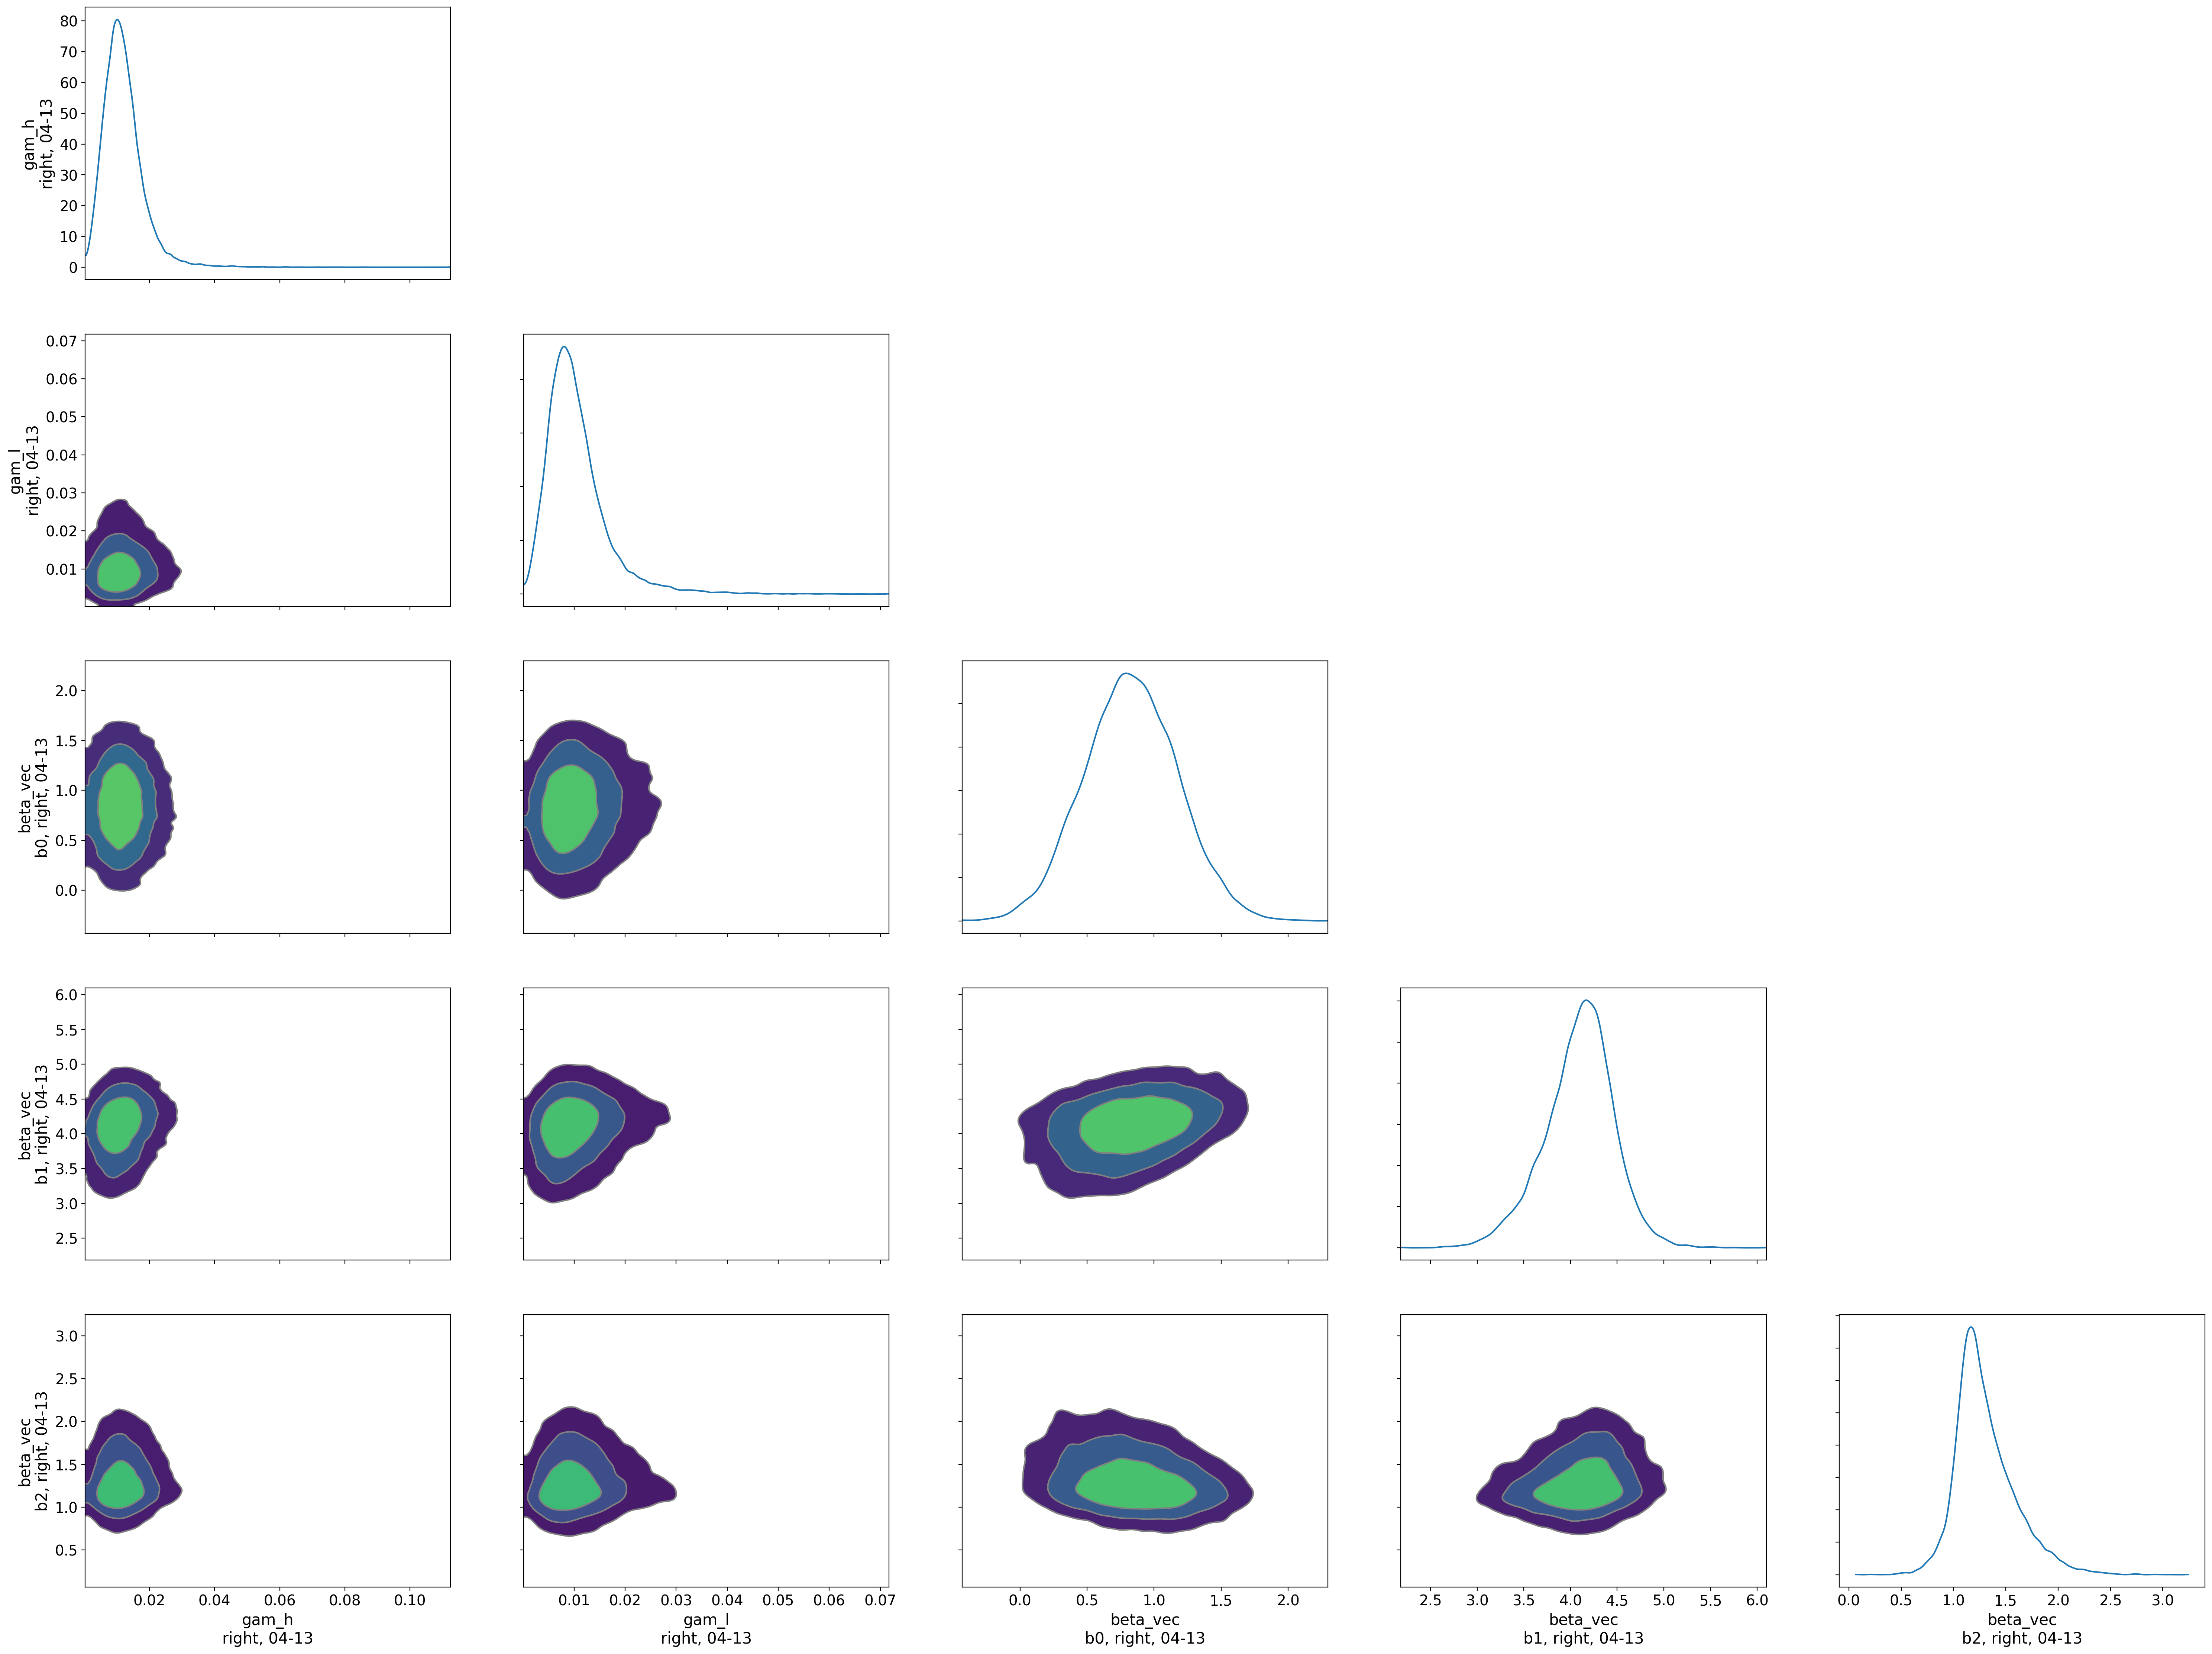
\includegraphics[width=0.85\textwidth]{pair_right_04-13.png}
\caption{As Figure~\ref{fig:pair_left}, for the right hand.}
\end{figure}

\begin{figure}[H]
\centering
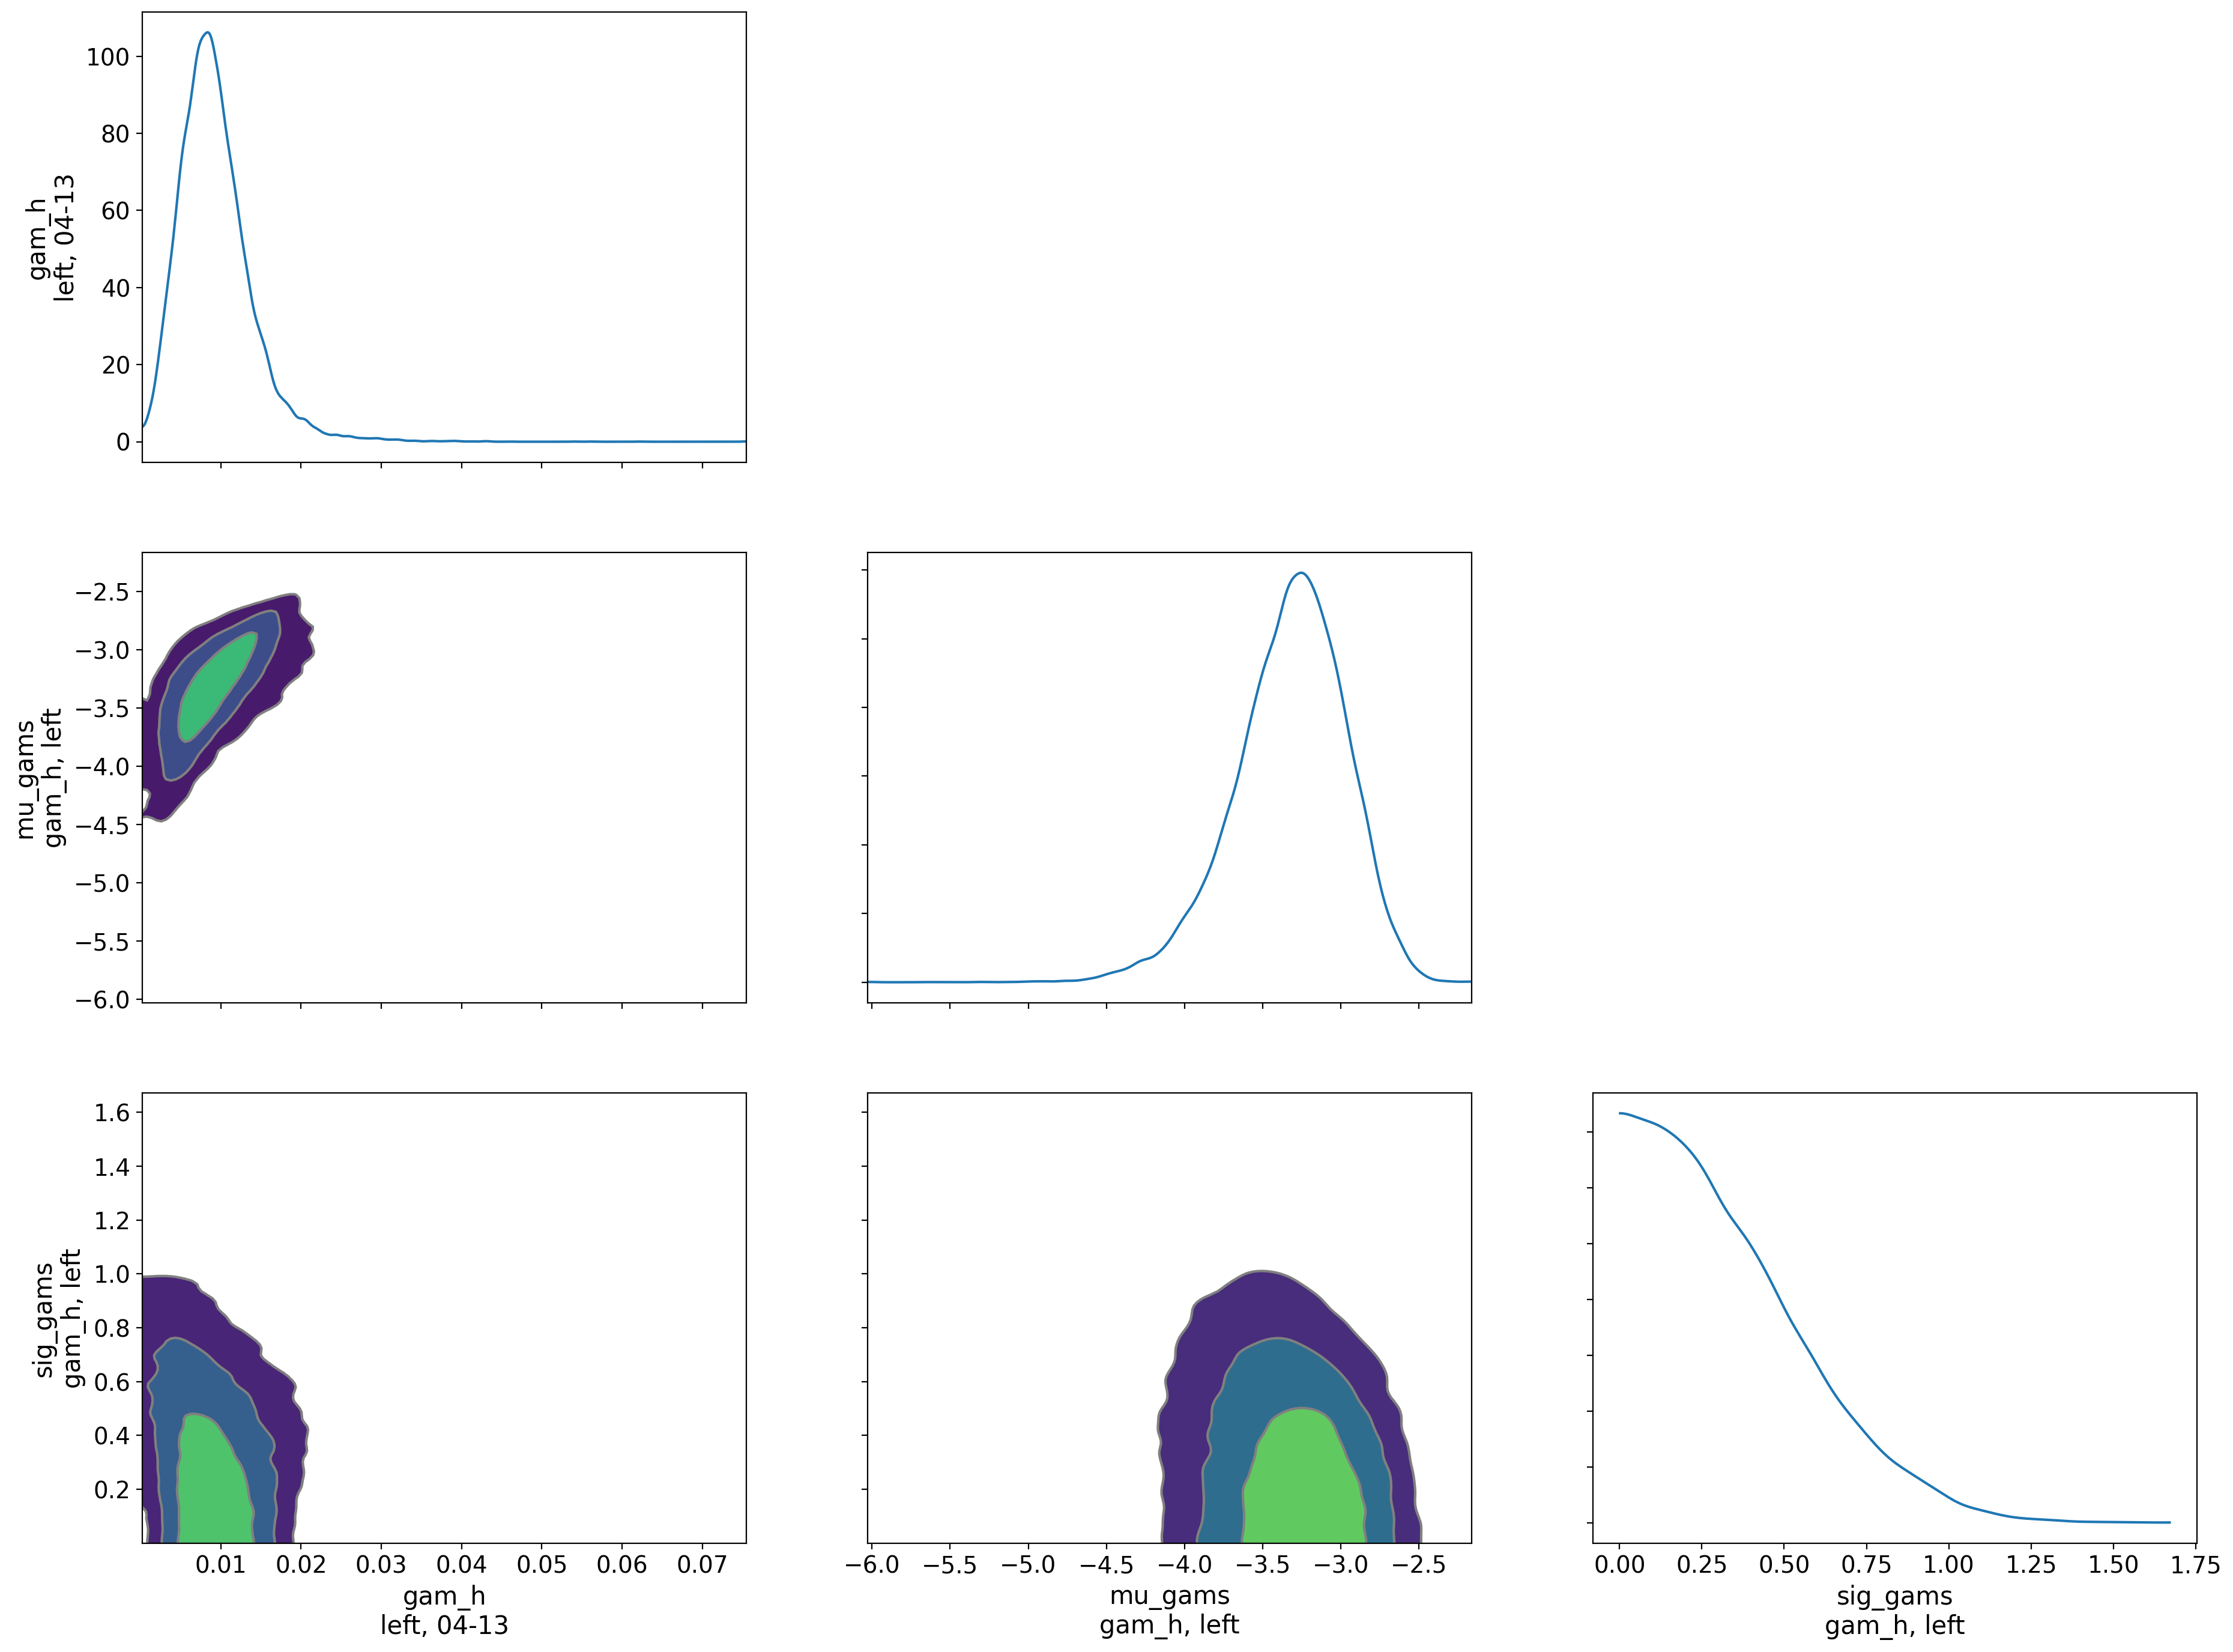
\includegraphics[width=0.75\textwidth]{pair_gam_h_hyper_left.png}
\caption{Joint posterior of the left hand's $\gamma_h$ on 04-13 and the
hyperparameters $\mu_{\gamma_h}$ and $\sigma_{\gamma_h}$.}
\label{fig:pair_hyper}
\end{figure}

\end{document}
